% !TeX program = pdflatex
% =============================================================================
% Arbeitsblatt: Zusammengesetzte Bewegungen (nicht bewertet, Übungsmaterial
% für den Unterricht)
% Kantonsschule KFR – Physik, 4. Klasse, 1. HS, Mechanik
%
% Kopiert aus vorlagen/arbeitsblatt-vorlage.tex und um dieselben
% Farb-/Boxdefinitionen ergänzt wie freier-fall-arbeitsblatt.tex /
% bewegungsgleichungen-arbeitsblatt.tex (gleicher Themencluster, direkt
% anschliessende Lektion). Templates sind selbstständig/nicht DRY, siehe
% CLAUDE.md.
%
% Notation: $v_{\text{rel}}$ (Eigengeschwindigkeit relativ zum Wasser/zur
% Luft), $v_{\text{Strömung}}$ (Strömungs-/Windgeschwindigkeit) und
% $v_{\text{ges}}$ (resultierende Geschwindigkeit über Grund) durchgehend für
% alle Fluss-/Windaufgaben, wie in lernziele.md vorgeschlagen.
%
% Vorhaltewinkel-Herleitung (LZ4): Zahlenwerte für das Theorie-Beispiel
% (Motorboot Rhein, b=180 m, Versatz=20 m, v_Strömung=1.5 m/s, v_rel=2.5 m/s)
% stammen 1:1 aus der in lernziele.md referenzierten Quelle
% "Beispiel_ Geschwindigkeit, Boot auf einem Fluss.pdf" und wurden gegen
% deren publizierte Zwischenresultate geprüft (β=83.66°, α=36.61°,
% v_ges=2.17 m/s, t=83.46 s). Die Limmat-Übungsaufgabe (b=40 m, Versatz=15 m,
% v_Strömung=0.6 m/s, v_rel=0.8 m/s) ist ein eigenes, unabhängig über die
% Vektorkomponenten UND über den Sinussatz gegengerechnetes Zahlenbeispiel
% (β≈69.4°, α≈44.6°, v_ges≈0.78 m/s, t≈54.8 s).
%
% Stand: Lernziele, Einleitung, Theorie und Aufgaben fertig (Reihenfolge =
% Dokumentreihenfolge, siehe Kommentar vor der Lernziele-infobox unten;
% stimmt hier mit der LZ-Nummerierung aus lernziele.md überein, keine
% Umnummerierung nötig).
% =============================================================================
\documentclass[addpoints,11pt,a4paper]{exam}

\usepackage[T1]{fontenc}
\usepackage[utf8]{inputenc}
\usepackage[ngerman]{babel}
\usepackage{lmodern}
\usepackage[a4paper,margin=2.2cm,headheight=14pt]{geometry}
\usepackage{amsmath}
\usepackage{amssymb}
\usepackage{siunitx}
% Hausstil: zusammengesetzte Einheiten immer als echter Bruch (\frac), nicht
% als Schrägstrich inline oder \tfrac. Gilt global für jedes \si/\SI.
\sisetup{per-mode=fraction,fraction-command=\frac}
\usepackage{array,booktabs,tabularx,multirow}
\usepackage{enumitem}
\usepackage{graphicx}
\usepackage{xcolor}
\usepackage{colortbl}
\usepackage{tikz}
\usepackage{physics}
\usepackage{circuitikz}
\usepackage[most]{tcolorbox}
\usepackage{lastpage}
\usepackage{needspace}
\usepackage{url}

\usetikzlibrary{arrows.meta,calc,angles,quotes}

\setlength{\parindent}{0pt}
\setlength{\parskip}{0.45em}

% -----------------------------
% Farben (Hausfarbschema Physik KFR)
% -----------------------------
\definecolor{titleblue}{HTML}{183A6B}
\definecolor{accentblue}{HTML}{2E6F9E}
\definecolor{lightblue}{HTML}{EAF4FB}
\definecolor{verylightblue}{HTML}{F7FBFE}
\definecolor{lightgray}{HTML}{F4F6F8}
\definecolor{darkgray}{HTML}{4A4A4A}
% Für Diagramme mit zwei verschiedenen Funktionen/Linien: titleblue (dunkles
% Blau) + accentorange (Orange) sind weit genug auseinander (auch in
% Graustufen/für Farbenblinde unterscheidbar), im Gegensatz zu
% titleblue+accentblue, die beide Blautöne sind.
\definecolor{accentorange}{HTML}{D9720C}
% Für Diagramme mit DREI Linien: dritte Farbe nötig, die sich sowohl von
% titleblue als auch von accentorange klar unterscheidet, auch in
% Graustufen/für Farbenblinde. Violett liegt weit genug von Blau und Orange
% entfernt, um als dritte Linie eindeutig unterscheidbar zu bleiben.
\definecolor{accentpurple}{HTML}{7B2D8E}
% Theorieblock: eigene Farbe (grün), damit er sich auf einen Blick von den
% blauen Lernziele-/Aufgaben-Boxen abhebt.
\definecolor{theorygreen}{HTML}{2E7D4F}
\definecolor{lighttheorygreen}{HTML}{EAF7EF}
% Gruppenarbeitbox: eigene Farbe (Petrol/Teal), damit Partner-/Gruppenarbeit
% sich auf einen Blick von normalen Einzelaufgaben (blau, taskbox) und vom
% Theorieblock (grün, theoriebox) abhebt.
\definecolor{groupteal}{HTML}{1B7F72}
\definecolor{lightgroupteal}{HTML}{E8F5F3}
% Vertiefungbox: eigene Farbe (gedecktes Bordeaux/Weinrot), NICHT dieselbe
% wie eine der übrigen Boxen, damit optionaler/fortgeschrittener Stoff
% (hier: der Sinussatz-Abschnitt zum Vorhaltewinkel) auf einen Blick als
% "das darf man auslassen" erkennbar ist, auch für Schüler, die nur die
% Randfarbe der Box sehen, ohne den Titeltext zu lesen.
\definecolor{vertiefungrot}{HTML}{8C2F39}
\definecolor{lightvertiefungrot}{HTML}{F7EAEC}

% -----------------------------
% Spaltentypen
% -----------------------------
\newcolumntype{Y}{>{\centering\arraybackslash}X}
\newcolumntype{P}[1]{>{\raggedright\arraybackslash}p{#1}}

% -----------------------------
% Boxen
% -----------------------------
\newtcolorbox{titlebox}{
  enhanced,
  colback=titleblue,
  colframe=titleblue,
  boxrule=0pt,
  arc=3mm,
  left=3mm,right=3mm,top=3mm,bottom=3mm
}

% exam.cls rückt die questions-Liste um die Breite von "10." (plus \labelsep)
% ein (Platz für die Nummerierung "1.", "2." ...); wir messen dieselbe Distanz
% hier unabhängig nach.
\newlength{\aufgabenindent}
\settowidth{\aufgabenindent}{10.\hskip\labelsep}

\newtcolorbox{infobox}{
  enhanced,
  breakable,
  colback=lightblue,
  colframe=accentblue,
  boxrule=0.7pt,
  arc=2mm,
  left=5mm,right=5mm,top=2mm,bottom=2mm
}

% theoriebox: wie infobox, aber grün und mit farbigem Titelbalken. Regel:
% hervorgehobene/definierte Begriffe INNERHALB einer theoriebox immer mit
% \textbf{\emph{...}} setzen (fett UND kursiv), nicht mit blossem \emph{...}.
\newtcolorbox{theoriebox}[1][Theorie]{
  enhanced,
  breakable,
  colback=lighttheorygreen,
  colframe=theorygreen,
  title={#1},
  fonttitle=\bfseries,
  boxrule=0.7pt,
  arc=2mm,
  left=5mm,right=5mm,top=2mm,bottom=2mm
}

% taskbox steht direkt in der questions-Liste (vor dem ersten \question),
% also innerhalb von deren Einrückung.
\newtcolorbox{taskbox}[1][]{
  enhanced,
  breakable,
  colback=verylightblue,
  colframe=accentblue,
  title={#1},
  fonttitle=\bfseries,
  boxrule=0.7pt,
  arc=2mm,
  enlarge left by=-\aufgabenindent,
  width=\textwidth,
  left=5mm,right=5mm,top=2mm,bottom=2mm
}

% beispielbox: wie taskbox (blau), aber ausserhalb von questions.
\newtcolorbox{beispielbox}[1][Beispiel]{
  enhanced,
  breakable,
  colback=verylightblue,
  colframe=accentblue,
  title={#1},
  fonttitle=\bfseries,
  boxrule=0.7pt,
  arc=2mm,
  left=5mm,right=5mm,top=2mm,bottom=2mm
}

% groupbox: JEDE Aufgabe mit Partner-/Gruppenarbeit bekommt diese Box statt
% der blauen taskbox. Strukturell identisch zu taskbox (gleiche
% Einrückungskorrektur, da auch groupbox innerhalb von questions steht).
\newtcolorbox{groupbox}[1][Gruppenarbeit]{
  enhanced,
  breakable,
  colback=lightgroupteal,
  colframe=groupteal,
  title={#1},
  fonttitle=\bfseries,
  boxrule=0.7pt,
  arc=2mm,
  enlarge left by=-\aufgabenindent,
  width=\textwidth,
  left=5mm,right=5mm,top=2mm,bottom=2mm
}

% hinweisbox: eigene Farbe (Orange), für wichtige Klarstellungen/Warnungen
% vor häufigen Verwechslungen.
\definecolor{lightorange}{HTML}{FCEEE0}
\newtcolorbox{hinweisbox}[1][Hinweis]{
  enhanced,
  breakable,
  colback=lightorange,
  colframe=accentorange,
  title={#1},
  fonttitle=\bfseries,
  boxrule=0.7pt,
  arc=2mm,
  left=5mm,right=5mm,top=2mm,bottom=2mm
}

% formelbox: eigene Farbe (Violett), um zentrale Formeln (Sinussatz,
% Pythagoras/Tangens im rechtwinkligen Geschwindigkeitsdreieck) visuell klar
% von normaler Theorie abzuheben.
\definecolor{lightpurple}{HTML}{F3EAF7}
\newtcolorbox{formelbox}[1][Formel]{
  enhanced,
  breakable,
  colback=lightpurple,
  colframe=accentpurple,
  title={#1},
  fonttitle=\bfseries,
  boxrule=0.9pt,
  arc=2mm,
  left=5mm,right=5mm,top=2mm,bottom=2mm
}

% vertiefungbox / vertiefungtaskbox: wie theoriebox/taskbox, aber in
% vertiefungrot statt grün/blau, für optionalen, fortgeschrittenen Stoff
% (Sinussatz-Abschnitt). vertiefungtaskbox steht wie taskbox/groupbox
% innerhalb von questions und braucht deshalb dieselbe
% Einrückungskorrektur; vertiefungbox steht wie theoriebox ausserhalb.
\newtcolorbox{vertiefungbox}[1][Vertiefung (optional)]{
  enhanced,
  breakable,
  colback=lightvertiefungrot,
  colframe=vertiefungrot,
  title={#1},
  fonttitle=\bfseries,
  boxrule=0.7pt,
  arc=2mm,
  left=5mm,right=5mm,top=2mm,bottom=2mm
}
\newtcolorbox{vertiefungtaskbox}[1][Vertiefung (optional)]{
  enhanced,
  breakable,
  colback=lightvertiefungrot,
  colframe=vertiefungrot,
  title={#1},
  fonttitle=\bfseries,
  boxrule=0.7pt,
  arc=2mm,
  enlarge left by=-\aufgabenindent,
  width=\textwidth,
  left=5mm,right=5mm,top=2mm,bottom=2mm
}

\newtcolorbox{answerbox}{
  breakable,
  colback=white,
  colframe=gray!55,
  boxrule=0.5pt,
  arc=1.5mm,
  left=2mm,right=2mm,top=2mm,bottom=2mm
}

% --- Lösungen ein-/ausblenden -----------------------------------------------
% Schülerexemplar (Standard): \noprintanswers
% Lehrer-/Lösungsexemplar:    \printanswers
\noprintanswers
% \printanswers

% --- Punkte bleiben intern, werden aber nicht gedruckt ----------------------
\pointformat{}

% --- Lösungsbox auf Deutsch, farblich abgesetzt -----------------------------
\renewcommand{\solutiontitle}{\noindent\color{titleblue}\textbf{Lösung:}\enspace}

% --- Kopf-/Fusszeile: Thema/Titel oben, Seitenzahl unten --------------------
\pagestyle{headandfoot}
\cfoot{\textcolor{darkgray}{Seite \thepage\ von \pageref{LastPage}}}

% --- Kopfzeile: Klasse / Datum / Thema / Titel ------------------------------
\newcommand{\Kopfzeile}[4]{%
  \begin{titlebox}
    {\color{white}\sffamily\bfseries\Large #4}
  \end{titlebox}
  \vspace{0.5em}
  \noindent\textbf{Klasse:}~#1 \hfill \textbf{Datum:}~#2 \hfill \textbf{Thema:}~#3
    \hfill \textbf{Lehrperson:}~Loris Keller
  \vspace{0.8em}
  \lhead{\textcolor{darkgray}{#3}}
  \rhead{\textcolor{darkgray}{#4}}
}

% --- Antwortraum: ca. 2.5 cm Platz pro Punkt, als umrandetes Feld -----------
\newlength{\antwortraumlen}
\newcommand{\Antwortraum}[1]{%
  \pgfmathsetlength{\antwortraumlen}{#1*2.5cm}%
  \begin{answerbox}
    \rule{0pt}{\antwortraumlen}%
  \end{answerbox}%
}

% Werte für Kopfzeile zentral setzen
\newcommand{\Klasse}{4a}
\newcommand{\Datum}{25.09.2026}
\newcommand{\Thema}{Zusammengesetzte Bewegungen}
\newcommand{\ArbeitsblattTitel}{Arbeitsblatt: Zusammengesetzte Bewegungen}

\begin{document}

\Kopfzeile{\Klasse}{\Datum}{\Thema}{\ArbeitsblattTitel}

% --- Lernziele: aus lernziele.md (Backward-Design, Stufe 1) übernommen.
% LZ1, LZ2, LZ3, LZ5 hier entsprechen der Reihenfolge, in der die
% zugehörigen Theorieboxen/Übungen im Dokument erscheinen. LZ4
% (Vorhaltewinkel/Sinussatz) ist bewusst ausgelassen: Der komplette
% Vertiefungsteil dazu ist aktuell per \iffalse...\fi auskommentiert (siehe
% Kommentar dort), lernziele.md behält die vollständige LZ1-LZ5-Nummerierung
% als Backward-Design-Referenz.
\begin{infobox}
\textbf{Lernziele}\\
Am Ende dieser Einheit kann ich \dots
\begin{itemize}[leftmargin=1.2cm,itemsep=0.25em]
  \item das Unabhängigkeitsprinzip erklären und an einem Beispiel anwenden. (LZ1)
  \item zwei Geschwindigkeitsvektoren grafisch addieren bzw. subtrahieren (Kopf-an-Schwanz-Methode). (LZ2)
  \item einen Vektor mit Sinus und Kosinus in seine Komponenten zerlegen und umgekehrt aus gegebenen Komponenten mit Pythagoras den Betrag und mit Tangens die Richtung des resultierenden Vektors berechnen. (LZ3)
  \item erklären, weshalb dieselbe Bewegung aus unterschiedlichen Bezugssystemen unterschiedlich aussehen kann, obwohl beide Beschreibungen korrekt sind. (LZ5)
\end{itemize}
\end{infobox}

% --- Einleitung: Regen-Hook (Bild aus Bilder/, SWR-Wissen-Grafik) statt des
% ursprünglichen reinen Zwei-Kugel-Gedankenexperiments. Führt direkt in die
% anschliessende Gruppenarbeit/Plenum-Diskussion. Knüpft weiterhin an die
% vorangegangene Freier-Fall-Einheit an ("g gilt für alle Objekte gleich"),
% wie in lernziele.md unter "Warum dieser Hook" begründet. -----------------
\begin{beispielbox}[Einleitung: Wirst du nasser, wenn du rennst?]
\begin{center}
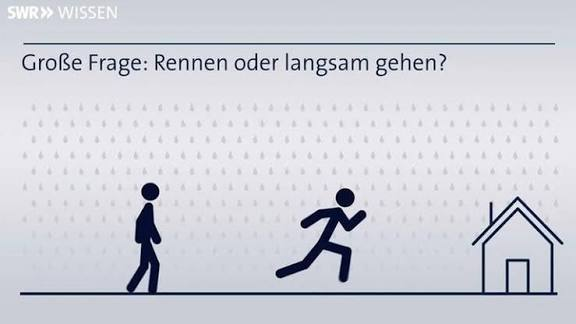
\includegraphics[width=0.65\linewidth]{Bilder/regen_laufen_vs_rennen.jpg}
\end{center}
{\scriptsize Grosse Frage: rennen oder gemütlich gehen, wenn es regnet?
(Quelle: SWR Wissen)}

Fast jeder kennt die Situation: Es fängt an zu regnen, und du musst noch
ein Stück zu Fuss zurücklegen. Rennst du los, oder gehst du gemütlich
weiter? Die naheliegende Antwort \glqq Rennen, dann bist du schneller aus
dem Regen\grqq{} ist nicht ganz so einfach, wie sie klingt: Beim Rennen
läufst du pro Sekunde auch in mehr Regentropfen hinein. Bevor du
weiterliest: Diskutiert die Frage gleich in der folgenden Gruppenarbeit.

Diese Frage hat mit genau dem Thema zu tun, das dieses Arbeitsblatt
behandelt: Was passiert, wenn gleichzeitig zwei Bewegungen wirken, eine
senkrechte (der fallende Regen) und eine waagrechte (deine eigene
Bewegung)? Genau das hast du in der letzten Einheit bereits für den freien
Fall kennengelernt: Alle Objekte fallen unabhängig von ihrer Masse gleich
schnell (Erdbeschleunigung $g$, siehe Hammer-Feder-Experiment auf dem
Mond). Diese Einheit erweitert diese Idee: Was, wenn zusätzlich zur
Fallbewegung noch eine zweite, \emph{gleichzeitige} Bewegung dazukommt?
\end{beispielbox}

% --- Gruppenarbeit + Plenum: Regen-Diskussion (ohne/mit Schirm), direkt zum
% Einleitungsbild. Bewusst als offene Diskussion ohne Musterlösung im Text
% (die Auflösung liefert das Video, von der Lehrperson im Plenum gezeigt),
% deshalb keine \begin{solution} bei den Diskussions-Parts. -----------------
\begin{groupbox}[Gruppenarbeit und Plenum: Gehen oder Rennen im Regen?]
\begin{parts}
  \part[2] \textbf{Gruppendiskussion (ohne Schirm):} Diskutiert zu dritt
  oder viert: Wirst du nasser, wenn du bei Regen rennst, oder wenn du
  gemütlich gehst, bei gleicher zurückgelegter Strecke? Sammelt Argumente
  für beide Seiten und einigt euch auf eine gemeinsame Vermutung mit
  Begründung.
  \Antwortraum{2}

  \part[1] \textbf{Plenum:} Vergleicht eure Vermutung mit den anderen
  Gruppen der Klasse. Gibt es unterschiedliche Meinungen? Woran könnte das
  liegen?
  \Antwortraum{1}

  \part[2] \textbf{Gruppendiskussion (mit Schirm):} Und wenn ihr einen
  Regenschirm dabei habt? Ändert sich eure Antwort, wenn ihr von oben
  geschützt seid? Diskutiert erneut in der Gruppe.
  \Antwortraum{2}

  \part[1] \textbf{Plenum:} Vergleicht auch diese Vermutung wieder mit der
  ganzen Klasse.
  \Antwortraum{1}
\end{parts}
\end{groupbox}

\begin{hinweisbox}[Auflösung im Video]
Die Lehrperson zeigt euch anschliessend im Plenum ein kurzes Video mit der
physikalischen Auflösung dieser Frage:
\url{https://www.swr.de/swrkultur/wissen/bei-regen-gehen-oder-rennen-wie-wird-man-weniger-nass-100.html}
\end{hinweisbox}

Genau dieselbe Unabhängigkeit von waagrechter und senkrechter Bewegung,
die im Video eine Rolle spielt, lässt sich mit einem einfachen
Tischexperiment direkt zeigen:

% --- Partnerarbeit: Predict-Observe-Explain-Linealexperiment für LZ1. Zwei
% Münzen, ein Lineal: klassischer, tatsächlich durchführbarer Schülerversuch
% (siehe Bilder/unabhaengigkeitsprinzip_schülerversuch.jpg), ersetzt das
% frühere, schwerer synchronisierbare Zwei-Münzen-Schnipp-Experiment. -------
\begin{groupbox}[Partnerarbeit: Das Linealexperiment]
\begin{center}
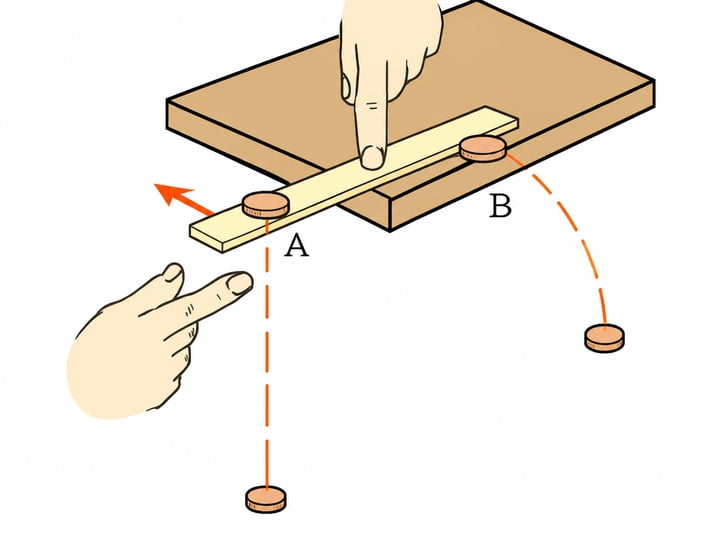
\includegraphics[width=0.55\linewidth]{Bilder/unabhaengigkeitsprinzip_schülerversuch.jpg}
\end{center}
{\scriptsize Münze A liegt auf dem über die Tischkante hinausragenden
Lineal, Münze B direkt daneben auf der Tischkante selbst. Wird das Lineal
blitzschnell weggezogen, fällt A praktisch senkrecht nach unten (gestrichelte
Linie links), während B einen waagrechten Wurf ausführt (gestrichelte
Bahn rechts).}

Ihr braucht zu zweit ein Lineal, zwei gleiche Münzen und eine Tischkante.

\begin{parts}
  \part[2] \textbf{Predict:} Legt ein Lineal so auf den Tisch, dass ein
  kurzes Stück über die Tischkante hinausragt. Legt eine Münze (A) auf
  dieses überstehende Stück. Legt eine zweite, gleiche Münze (B) direkt
  daneben auf die Tischkante selbst, nicht auf das Lineal (siehe Bild).
  Notiert zuerst, ohne es auszuprobieren, eure Vorhersage: Was passiert mit
  A und B, wenn ihr das Lineal blitzschnell und kräftig unter Münze A
  wegzieht? Kommen beide gleichzeitig am Boden an?
  \Antwortraum{2}

  \part[1] \textbf{Observe:} Zieht das Lineal mehrmals blitzschnell weg
  (ein kurzer, kräftiger Ruck, kein langsames Herausziehen) und beobachtet
  genau, was mit A und B passiert.
  \Antwortraum{1}

  \needspace{10.5cm}
  \part[3] \textbf{Explain:} Stimmt eure Beobachtung mit eurer Vorhersage
  überein? Münze A fällt praktisch senkrecht nach unten (freier Fall),
  Münze B wird vom wegschnellenden Lineal seitlich angestossen und fliegt
  einen waagrechten Bogen (waagrechter Wurf). Erklärt: Warum kommen
  trotzdem beide Münzen gleichzeitig auf dem Boden an?
  \Antwortraum{3}
  \begin{solution}
  Beide Münzen kommen gleichzeitig auf dem Boden an. Die waagrechte
  Wurfbewegung von B und die senkrechte Fallbewegung beeinflussen sich
  \textbf{nicht}: Auf beide Münzen wirkt exakt dieselbe Erdbeschleunigung
  $g$ senkrecht nach unten, völlig unabhängig davon, ob sich eine Münze
  zusätzlich noch waagrecht bewegt. Münze B legt in derselben Zeit einfach
  zusätzlich eine grosse waagrechte Strecke zurück, das ändert aber nichts
  an ihrer Fallzeit. Das ist dasselbe Prinzip, das ihr schon aus der
  Einheit zum freien Fall kennt (\glqq $g$ gilt für alle Objekte
  gleich\grqq{}), jetzt nur erweitert um eine zusätzliche, unabhängige
  Bewegung zur Seite.
  \end{solution}
\end{parts}
\end{groupbox}

% =============================================================================
% Diagnostische Sortieraufgabe (C1): aktiviert das mathematische
% Vektor-Vorwissen, bevor irgendeine neue Theorie eingeführt wird. Keine
% eigene LZ-Nummer (reine Aktivierungsaufgabe), siehe lernziele.md.
% =============================================================================
\begin{questions}
\begin{taskbox}[Sortieraufgabe: Eine oder zwei Bewegungsrichtungen?]
\question[11] Für jede der folgenden Situationen: Findet die Bewegung
\textbf{entlang einer einzigen Linie} statt (\glqq 1D\grqq{}), oder wirken
\textbf{zwei unterschiedliche Richtungen gleichzeitig} (\glqq 2D\grqq{})?
Kreuzt jeweils an. Einige Situationen sind bewusst trickreich, lest also
genau. Ihr müsst noch nichts berechnen können, nur einordnen, das braucht
ihr erst später in diesem Arbeitsblatt.

\begin{parts}
  \part[1] Ein Velo fährt bei völliger Windstille eine gerade Strasse
  hinunter.
  \begin{itemize}[leftmargin=1.2cm,itemsep=0.1em]
    \item[$\square$] 1D \hfill $\square$ 2D
  \end{itemize}

  \part[1] Eine Schwimmerin schwimmt schräg gegen die Strömung, um trotz
  Fluss exakt gegenüber ihrem Startpunkt anzukommen.
  \begin{itemize}[leftmargin=1.2cm,itemsep=0.1em]
    \item[$\square$] 1D \hfill $\square$ 2D
  \end{itemize}

  \part[1] Ein Fallschirmspringer fällt bei völliger Windstille senkrecht
  nach unten.
  \begin{itemize}[leftmargin=1.2cm,itemsep=0.1em]
    \item[$\square$] 1D \hfill $\square$ 2D
  \end{itemize}

  \part[1] Ein Zug fährt mit konstantem Tempo auf gerader Strecke (keine
  Kurve, keine Steigung).
  \begin{itemize}[leftmargin=1.2cm,itemsep=0.1em]
    \item[$\square$] 1D \hfill $\square$ 2D
  \end{itemize}

  \part[1] Regentropfen fallen bei böigem Wind schräg, für eine
  stillstehende Person am Boden betrachtet.
  \begin{itemize}[leftmargin=1.2cm,itemsep=0.1em]
    \item[$\square$] 1D \hfill $\square$ 2D
  \end{itemize}

  \part[1] Eine Kugel wird schräg nach oben geworfen (weder senkrecht noch
  waagrecht).
  \begin{itemize}[leftmargin=1.2cm,itemsep=0.1em]
    \item[$\square$] 1D \hfill $\square$ 2D
  \end{itemize}

  \part[1] Eine Person geht auf einer fahrenden Rolltreppe zusätzlich noch
  seitwärts, um jemanden zu überholen.
  \begin{itemize}[leftmargin=1.2cm,itemsep=0.1em]
    \item[$\square$] 1D \hfill $\square$ 2D
  \end{itemize}

  \part[1] Ein Skifahrer fährt exakt in der Falllinie einen Hang hinunter,
  ohne seitlich zu schwingen.
  \begin{itemize}[leftmargin=1.2cm,itemsep=0.1em]
    \item[$\square$] 1D \hfill $\square$ 2D
  \end{itemize}

  \part[1] Ein Ball wird in einem stillstehenden Zug senkrecht hochgeworfen.
  \begin{itemize}[leftmargin=1.2cm,itemsep=0.1em]
    \item[$\square$] 1D \hfill $\square$ 2D
  \end{itemize}

  \part[2] Ein Fallschirmspringer fällt senkrecht (Windstille), jetzt aber
  aus Sicht eines Piloten betrachtet, der mit konstantem Tempo waagrecht
  über ihm vorbeifliegt.
  \begin{itemize}[leftmargin=1.2cm,itemsep=0.1em]
    \item[$\square$] 1D \hfill $\square$ 2D
  \end{itemize}
  \Antwortraum{1}
  \begin{solution}
  a) 1D (geradeaus, ohne Wind keine zweite Richtung im Spiel). \quad
  b) 2D (Vorhaltewinkel: die Eigengeschwindigkeit zeigt schräg, dazu kommt
  die Strömung). \quad
  c) 1D (nur senkrecht, kein Wind lenkt ihn zur Seite ab). \quad
  d) 1D (gerade Strecke, konstantes Tempo, keine zweite Richtung). \quad
  e) 2D (senkrechter Fall und waagrechte Windbewegung gleichzeitig, anders
  als bei c) und im Gegensatz zur windstillen Version dieser Situation aus
  der Einleitung). \quad
  f) 2D (schiefer Wurf: eine waagrechte und eine senkrechte Komponente
  gleichzeitig, wie beim Zwei-Kugel-Experiment, nur mit einer zusätzlichen
  Anfangsgeschwindigkeit schräg nach oben statt nur waagrecht). \quad
  g) 2D (die Rolltreppenbewegung und die seitliche Zusatzbewegung liegen
  \emph{nicht} mehr auf derselben Linie, anders als beim einfachen
  Mitgehen). \quad
  h) 1D (die ganze Bewegung liegt auf der Falllinie, keine zweite Richtung
  kommt dazu). \quad
  i) 1D (ganz normaler senkrechter Wurf, wie in der letzten Einheit). \quad
  j) 2D: Aus Sicht des Piloten kommt zur senkrechten Fallbewegung noch die
  waagrechte Relativgeschwindigkeit zwischen Flugzeug und Fallschirmspringer
  dazu, genau wie beim Ball im Zug (aus Sicht der Person am Bahndamm), den du
  weiter unten in diesem Arbeitsblatt noch genauer kennenlernst. Aus Sicht
  einer Person am Boden wäre es dagegen weiterhin 1D, siehe Antwort c).
  Genau diese Doppelantwort, je nach Bezugssystem, klärst du ganz am Ende
  dieses Arbeitsblatts genauer.
  \end{solution}
\end{parts}
\end{taskbox}
\end{questions}

% =============================================================================
% Theorie: fachliche Grundlage für die Aufgaben, in eigene Boxen unterteilt,
% Reihenfolge = Lernzielreihenfolge oben.
% =============================================================================
\begin{theoriebox}[Das Unabhängigkeitsprinzip]
Führt ein Körper \textbf{\emph{gleichzeitig mehrere Bewegungen}} aus (zum
Beispiel eine waagrechte und eine senkrechte), so beeinflussen sich diese
gegenseitig \textbf{\emph{nicht}}. Man nennt das das
\textbf{\emph{Unabhängigkeitsprinzip der Bewegungen}}: Jede
Geschwindigkeitskomponente verhält sich so, als gäbe es die andere gar
nicht, und die Gesamtbewegung ergibt sich, indem man die Komponenten
anschliessend wieder zusammensetzt (addiert).

Das Zwei-Münzen-Experiment von eben ist ein direktes Beispiel: Die
waagrechte Stossbewegung und die senkrechte Fallbewegung sind vollständig
unabhängig voneinander. Dieselbe Überlegung gilt zum Beispiel für einen
Schwimmer, der sich relativ zum Wasser bewegt, während ihn gleichzeitig die
Strömung mitnimmt: Beide Bewegungen wirken unbeeinflusst voneinander, vom
Ufer aus gesehen addieren sie sich einfach zu einer Gesamtbewegung.

\begin{hinweisbox}
Mit \glqq mehreren Bewegungen\grqq{} ist \textbf{nicht} gemeint, dass ein
Gegenstand auseinanderbricht und in verschiedene Richtungen wegfliegt.
Gemeint ist, dass sich die Geschwindigkeit als Vektor in Komponenten
zerlegen und wieder zusammensetzen lässt, und dass diese Komponenten sich
beim Zusammensetzen nicht gegenseitig verändern.
\end{hinweisbox}
\end{theoriebox}

% =============================================================================
% Anwendung von LZ1: Regenschirm-Rand-Aufgabe, direkter Bezug zur
% Einleitungs-Diskussion (Gehen/Rennen im Regen). Rein qualitatives,
% idealisiertes Einzeltropfen-Modell (kein Wind, v0=0 beim Fallbeginn);
% beantwortet bewusst nur EINEN Teilaspekt der Diskussionsfrage und verweist
% explizit zurück auf Video/Diskussion für das Gesamtbild, siehe
% lernziele.md-Abgrenzung (keine quantitative Wurfparabel-Konstruktion
% nötig, nur freier Fall + Vergleich zweier Zeiten/Strecken).
% =============================================================================
\begin{questions}
\begin{taskbox}[Übung: Der Regenschirmrand]
\begin{center}
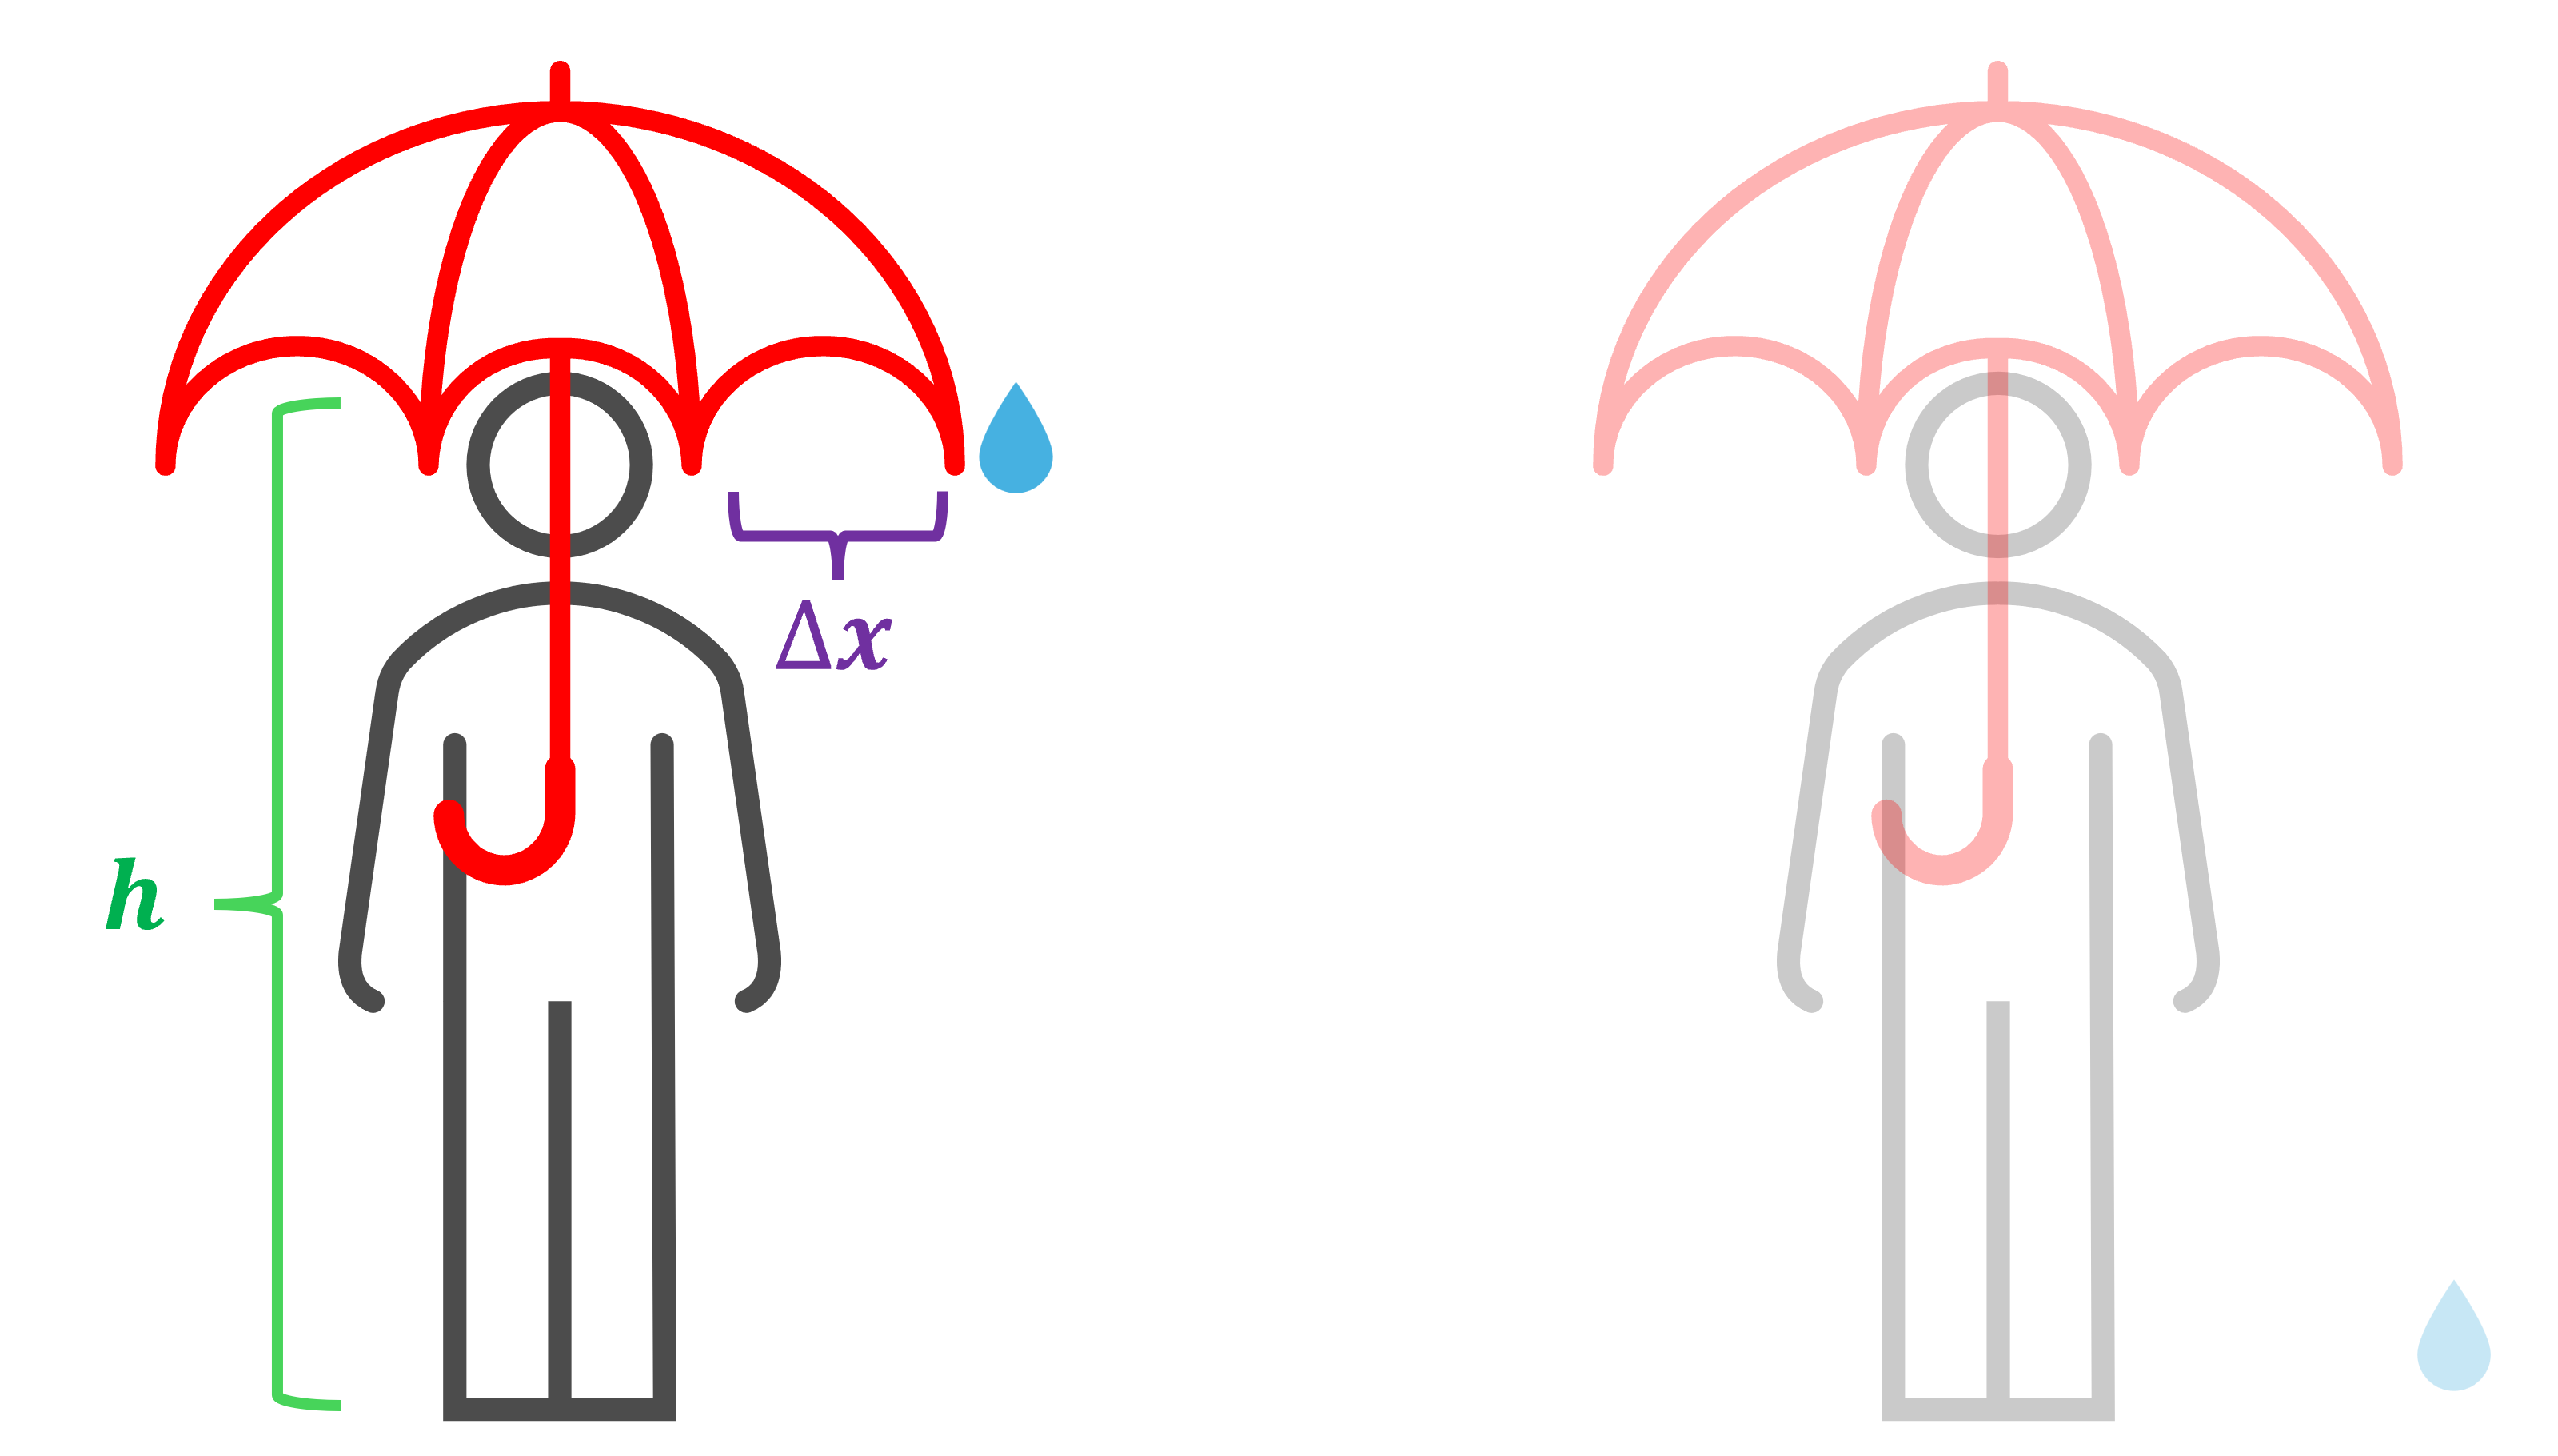
\includegraphics[width=0.32\linewidth]{Bilder/Regenschirm_Stehen.png}
\end{center}
{\scriptsize Zwei Momentaufnahmen: Links beginnt der Tropfen auf Höhe
$h$, im Abstand $\Delta x$ von dir, zu fallen. Rechts ist er am Boden
angekommen. Bewegst du dich in der Zwischenzeit nicht, bleibt der
Abstand $\Delta x$ unverändert, denn der Tropfen fällt rein senkrecht.}

\question[6] Du gehst bei Regen unter einem Regenschirm. Der vordere
Schirmrand ist in Gehrichtung immer um $\Delta x=\SI{0.4}{\meter}$ weiter
vorne als du selbst, auf einer Höhe von $h=\SI{1.6}{\meter}$ über dem
Boden. Ein Regentropfen, der sich gerade genau am vorderen Schirmrand
befindet (Höhe $h$, kein Wind), beginnt in diesem Moment frei zu fallen.

\begin{parts}
  \part[3] Berechne, wie lange der Tropfen braucht, um von der
  Schirmrandhöhe $h$ auf den Boden zu fallen (freier Fall aus der Ruhe,
  wie in der letzten Einheit).
  \Antwortraum{3}
  \begin{solution}
  \[
    t = \sqrt{\frac{2h}{g}} = \sqrt{\frac{2\cdot\SI{1.6}{\meter}}{\SI{9.81}{\meter\per\second\squared}}} \approx \sqrt{\SI{0.326}{\second\squared}} \approx \SI{0.571}{\second}.
  \]
  \end{solution}

  \part[3] Du selbst brauchst bei Geschwindigkeit $v$ die Zeit
  $\tau=\Delta x/v$, um den Schirmrand zu erreichen (Unabhängigkeitsprinzip:
  deine waagrechte Bewegung und der senkrechte Fall des Tropfens
  beeinflussen sich nicht, du kannst beide Zeiten getrennt berechnen und
  vergleichen). Berechne die \textbf{\emph{kritische Geschwindigkeit}}
  $v_{\text{krit}}$, bei der du genau in dem Moment am Schirmrand
  ankommst, in dem der Tropfen den Boden erreicht ($\tau=t$).

  \begin{center}
  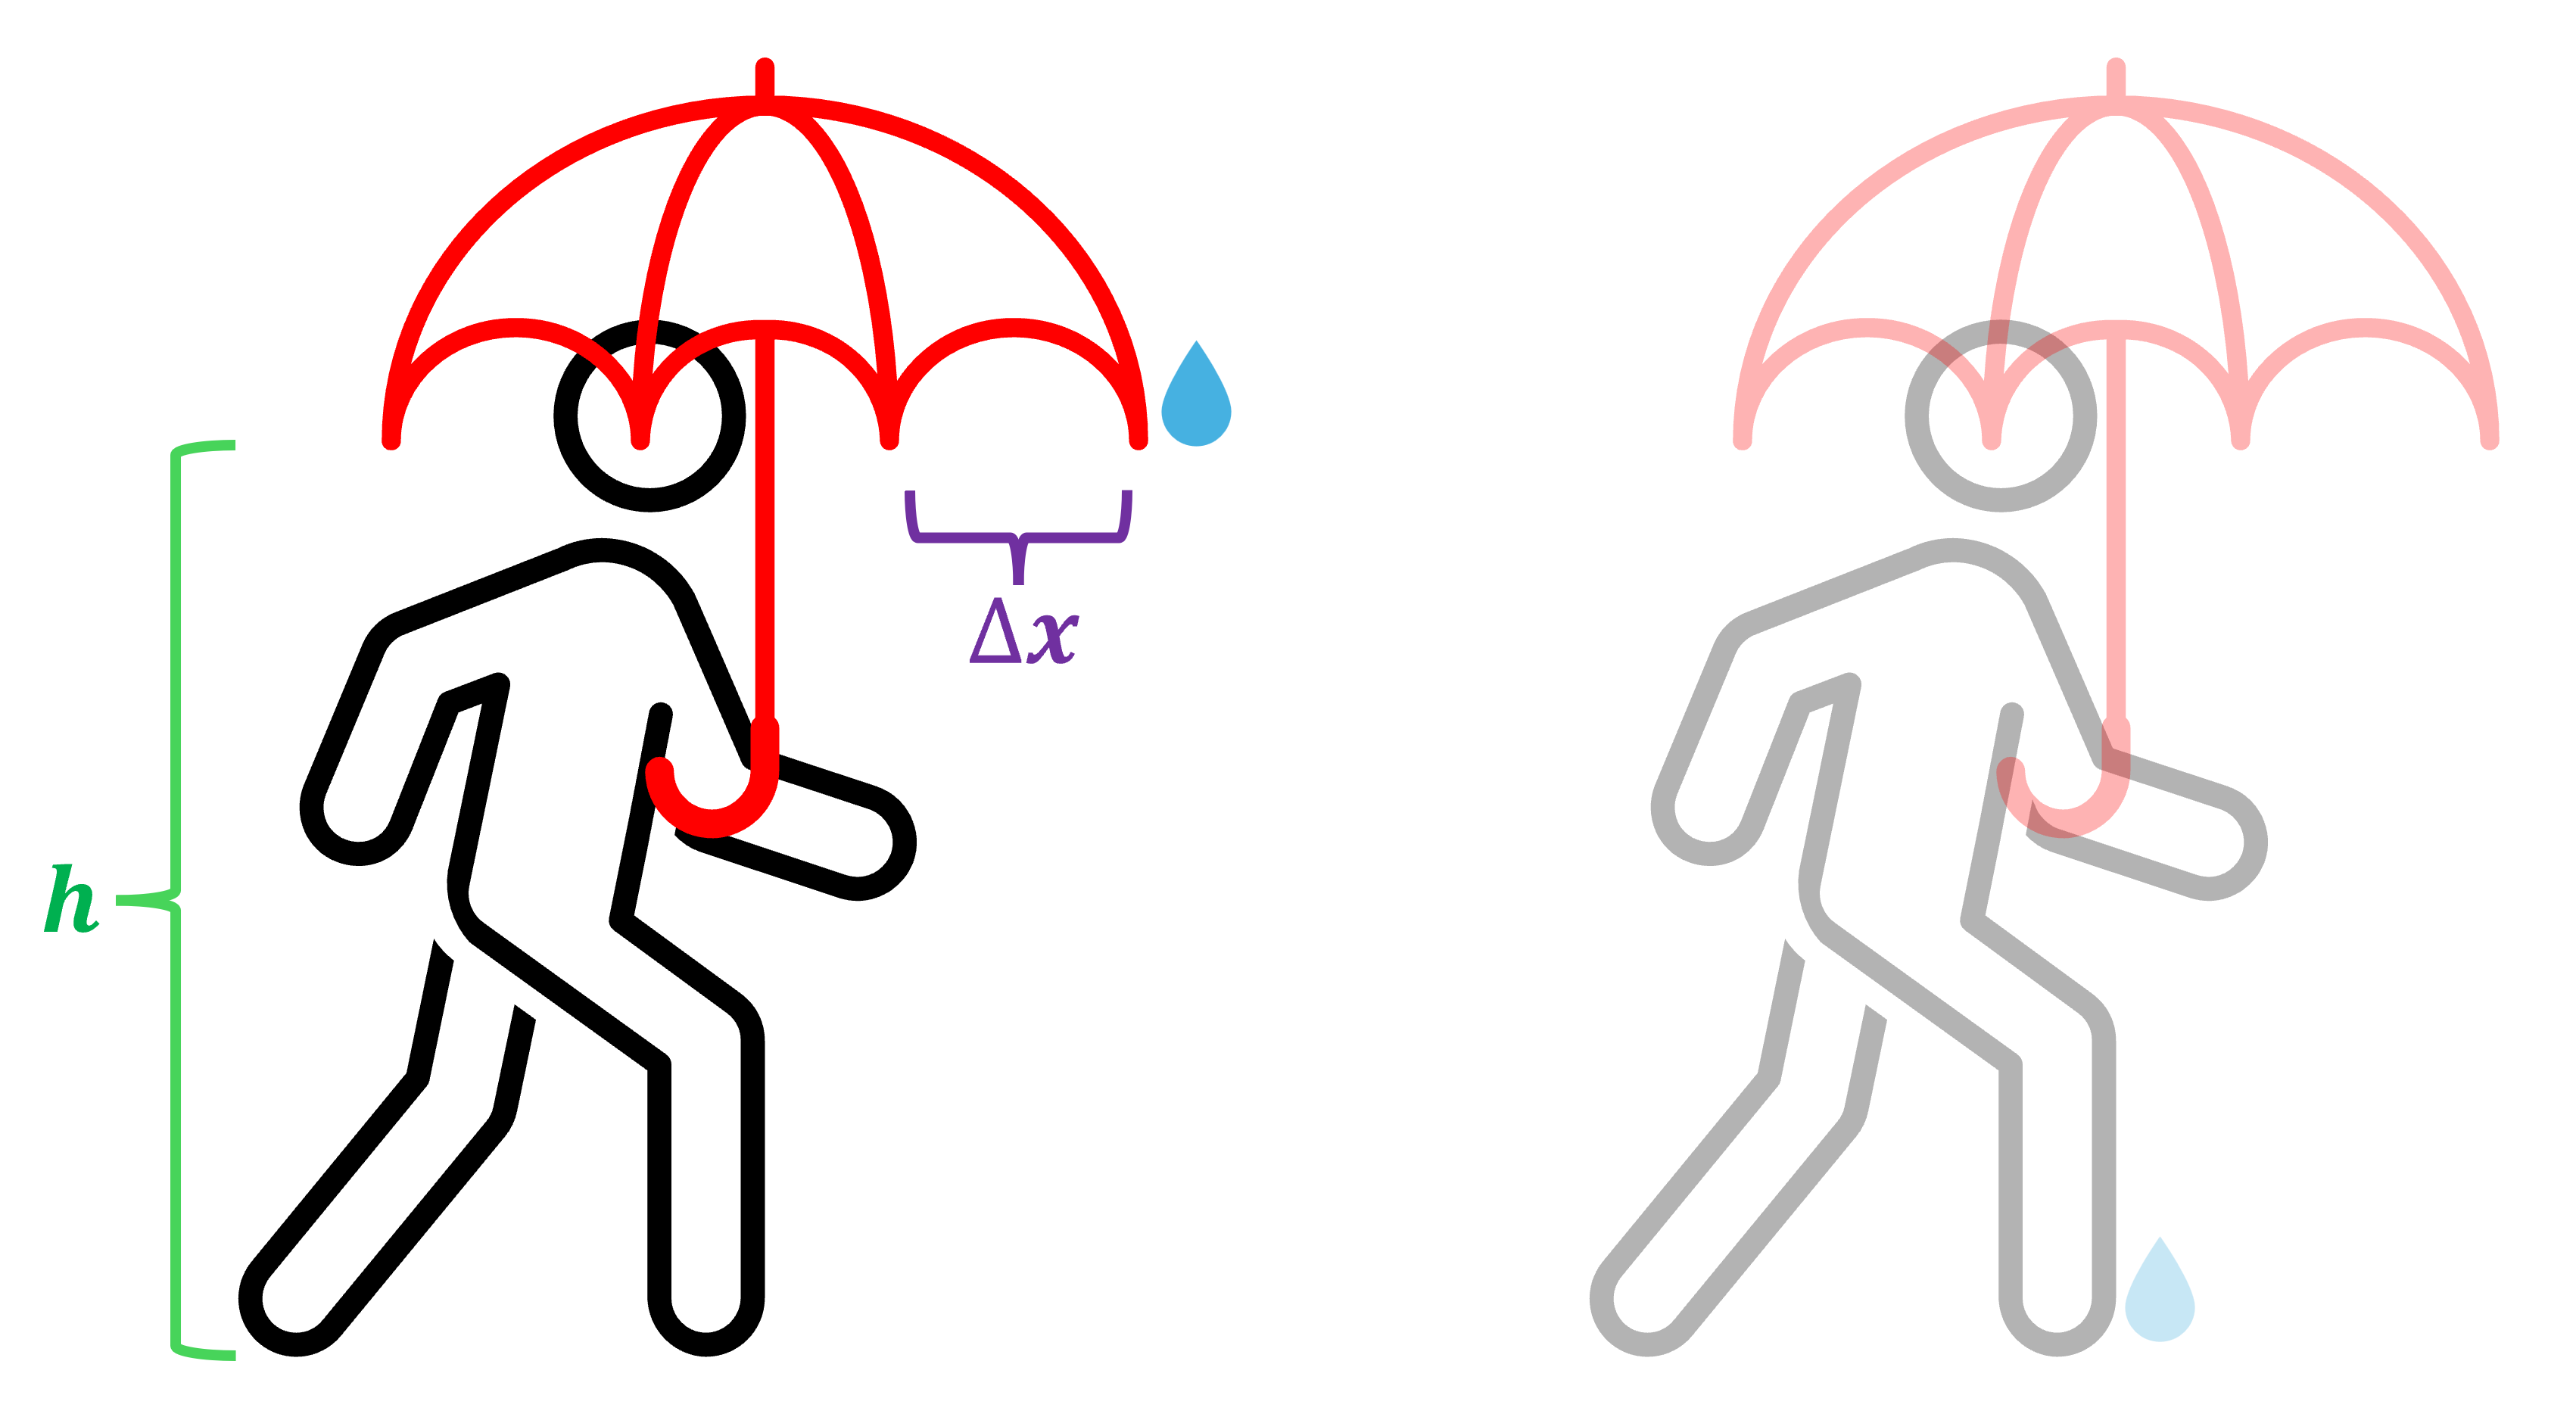
\includegraphics[width=0.36\linewidth]{Bilder/Regenschirm_Laufen.png}
  \end{center}
  {\scriptsize Zwei Momentaufnahmen bei $v_{\text{krit}}$: Links beginnt
  der Tropfen am Schirmrand zu fallen, rechts kommst du genau in dem
  Moment an, in dem er den Boden erreicht.}
  \Antwortraum{3}
  \begin{solution}
  \[
    v_{\text{krit}} = \frac{\Delta x}{t} = \frac{\SI{0.4}{\meter}}{\SI{0.571}{\second}} \approx \SI{0.70}{\meter\per\second}.
  \]
  \end{solution}
\end{parts}

\begin{hinweisbox}[Überraschung: langsamer ist hier sicherer]
Bist du \textbf{\emph{langsamer}} als $v_{\text{krit}}$, brauchst du für
$\Delta x$ \emph{länger} als $t$: Der Tropfen ist dann schon am Boden
aufgeschlagen, bevor du überhaupt am Schirmrand ankommst, du gehst sicher
an der Stelle vorbei. Bist du dagegen \textbf{\emph{schneller}} als
$v_{\text{krit}}$, bist du \emph{vor} dem Tropfen am Schirmrand und läufst
geradewegs in seine Fallbahn hinein. Für \textbf{\emph{diesen einen}}
Tropfen gilt also: Je schneller du gehst, desto eher holst du ihn ein,
statt ihm zu entkommen.
\end{hinweisbox}

\question[6] Du gehst tatsächlich mit deinem normalen Gehtempo
$v=\SI{1.4}{\meter\per\second}$.

\begin{parts}
  \part[3] Wie weit vom Schirmrand entfernt dürfte ein Regentropfen (auf
  Schirmhöhe $h$) höchstens \emph{starten}, damit du ihn bei diesem Tempo
  noch \glqq einholst\grqq{}, bevor er den Boden erreicht? Nenne diese
  maximale Startdistanz $d$.

  \begin{center}
  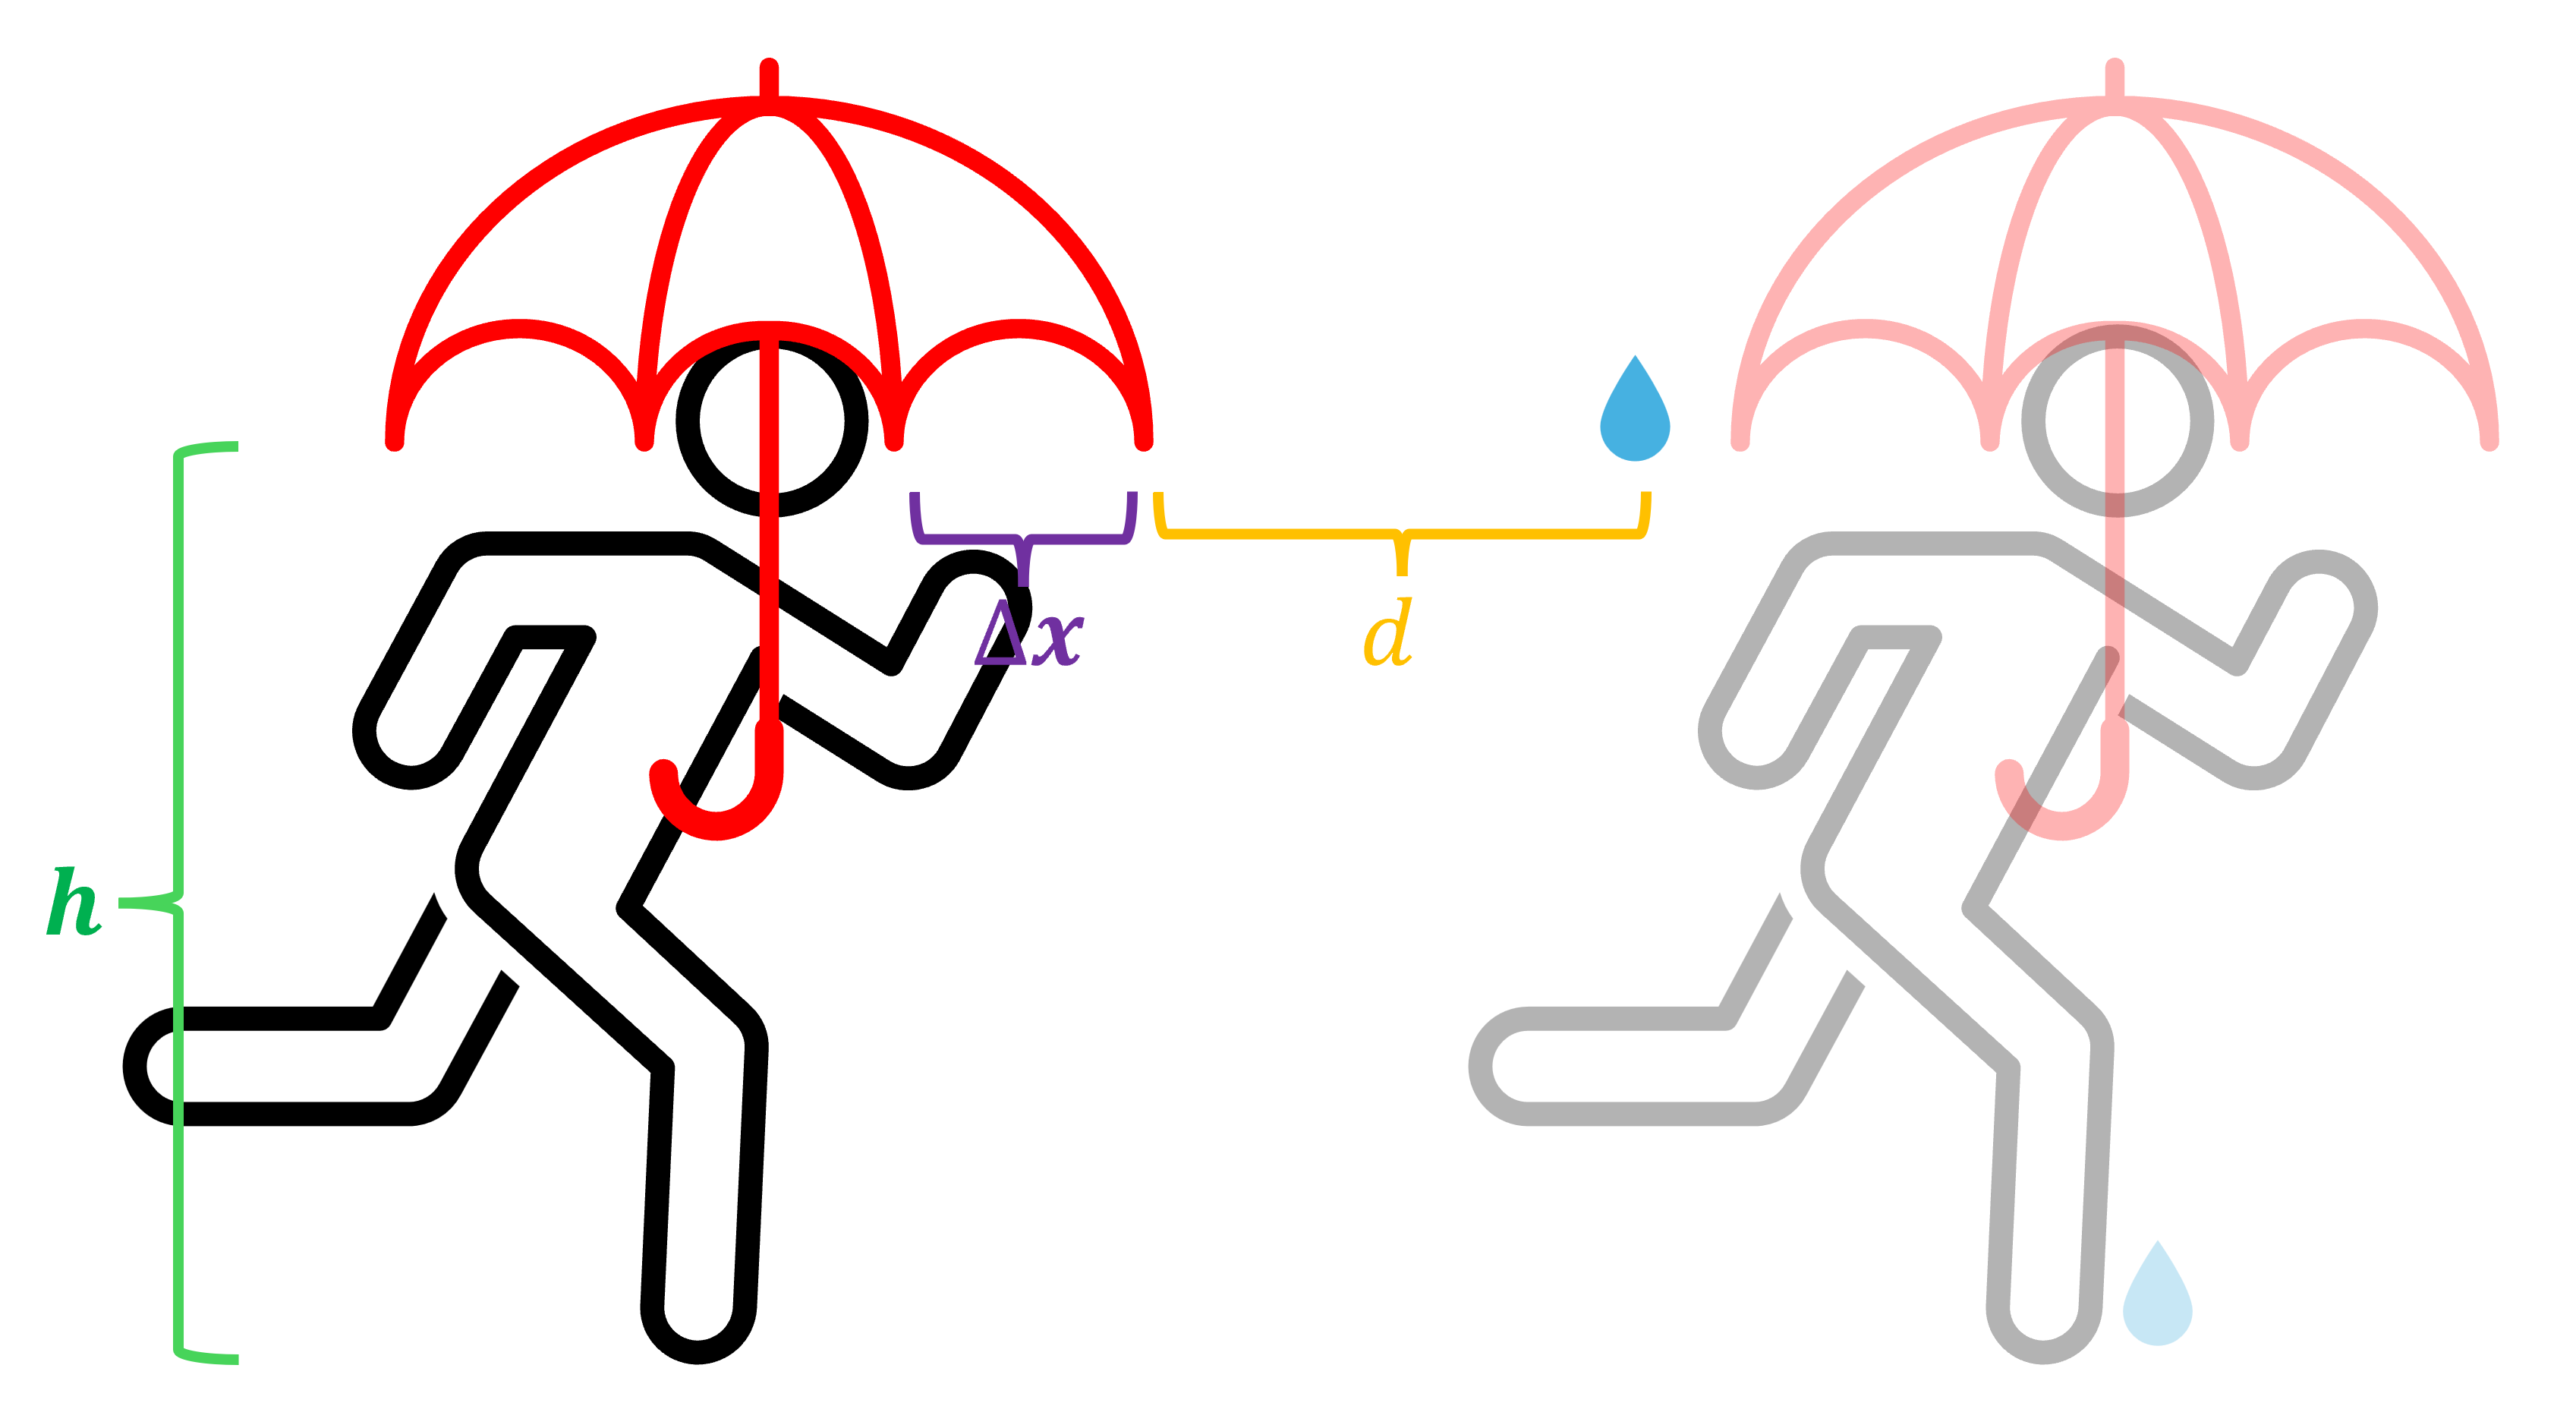
\includegraphics[width=0.42\linewidth]{Bilder/Regenschirm_Rennen.png}
  \end{center}
  {\scriptsize Zwei Momentaufnahmen: Links startet der Tropfen im
  maximal möglichen Abstand $d$ vom Schirmrand, rechts erreichst du
  genau noch die Stelle, an der er landet.}
  \Antwortraum{3}
  \begin{solution}
  \[
    d = v\cdot t = \SI{1.4}{\meter\per\second}\cdot\SI{0.571}{\second} \approx \SI{0.80}{\meter}.
  \]
  Der tatsächliche Schirmvorsprung ($\Delta x=\SI{0.4}{\meter}$) liegt
  \emph{innerhalb} dieser Zone ($\SI{0.4}{\meter}<\SI{0.80}{\meter}$): Bei
  normalem Gehtempo bist du schneller am Schirmrand als der Tropfen am
  Boden, du holst ihn also im Weitergehen buchstäblich ein. Erst ein
  deutlich langsameres Tempo, unter $v_{\text{krit}}\approx
  \SI{0.70}{\meter\per\second}$ aus Aufgabe 1, würde dich vor genau diesem
  Tropfen schützen.
  \end{solution}

  \part[2] Eine dritte Person rennt stattdessen mit
  $v=\SI{3.0}{\meter\per\second}$. Berechne für sie die maximale
  Startdistanz $d$.
  \Antwortraum{2}
  \begin{solution}
  \[
    d = \SI{3.0}{\meter\per\second}\cdot\SI{0.571}{\second} \approx \SI{1.71}{\meter}.
  \]
  \end{solution}

  \part[1] Wächst die so \glqq einholbare Zone\grqq{} (die möglichen
  Startpositionen eines Tropfens, den du auf diese Art noch einholst) mit
  steigender Geschwindigkeit, oder schrumpft sie?
  \Antwortraum{1}
  \begin{solution}
  Sie wächst: $d=v\cdot t$ ist proportional zu $v$. Schneller gehen oder
  rennen vergrössert also sogar die Zone, aus der du einen Tropfen auf
  diese Weise noch einholen könntest. Das entscheidet aber nicht allein,
  wer insgesamt trockener bleibt: Das hängt von der \emph{gesamten
  Anzahl} Tropfen ab, die dich während der ganzen Strecke treffen, nicht
  nur von dieser einen Randzone, siehe Video und Diskussion oben.
  \end{solution}
\end{parts}
\end{taskbox}
\end{questions}

\begin{theoriebox}[Vektoren grafisch addieren und subtrahieren: Kopf-an-Schwanz]
Um herauszufinden, welche Gesamtgeschwindigkeit bei zwei gleichzeitigen
Bewegungen herauskommt, addiert man ihre Geschwindigkeitsvektoren. Das geht
grafisch mit der \textbf{\emph{Kopf-an-Schwanz-Methode}}: Man zeichnet den
ersten Vektor, setzt den zweiten Vektor genau an dessen Spitze (\glqq
Kopf\grqq{}) an, ohne seine Länge oder Richtung zu verändern, und zieht dann
einen neuen Pfeil vom Startpunkt des ersten bis zur Spitze des zweiten
Vektors. Dieser neue Pfeil ist der \textbf{\emph{resultierende Vektor}} (die
Summe). Eine \textbf{\emph{Subtraktion}} $\vec{v}_1-\vec{v}_2$ funktioniert
genau gleich, nur dass man statt $\vec{v}_2$ den \textbf{\emph{umgekehrten}}
Vektor $-\vec{v}_2$ (gleiche Länge, entgegengesetzte Richtung)
Kopf-an-Schwanz anhängt.

\begin{hinweisbox}[Massstab: So zeichnest du exakt]
Jede Zeichnung in diesem Abschnitt hat einen angegebenen
\textbf{\emph{Massstab}} (zum Beispiel $\SI{1}{\centi\meter}\;\widehat{=}\;
\SI{1}{\meter\per\second}$): Die Länge eines Pfeils auf dem Papier
entspricht direkt der Geschwindigkeit. \textbf{\emph{Bevor du zu messen
beginnst:}} Ein Ausdruck oder eine Kopie kann leicht vom Original
abweichen, zum Beispiel durch den Drucker. Miss deshalb zuerst mit deinem
Lineal den Abstand zwischen zwei benachbarten Gitterlinien auf
\emph{deinem} Blatt nach. Dieser gemessene Abstand entspricht laut Angabe
genau einer Einheit (im Beispiel oben: $\SI{1}{\meter\per\second}$), auch
wenn er nicht exakt $\SI{1}{\centi\meter}$ misst. Rechne mit dieser
tatsächlich gemessenen Länge weiter, nicht mit dem angegebenen
Nominalwert. Zeigt ein Vektor nicht exakt waagrecht oder senkrecht, kannst
du seine Richtung trotzdem exakt zeichnen: Miss den gegebenen Winkel mit
dem \textbf{\emph{Geodreieck}} ab und trage die passende Länge (in deiner
tatsächlich gemessenen Einheit) in dieser Richtung ab. So funktioniert die
Methode für \textbf{\emph{jeden}} Vektor, unabhängig davon, in welche
Richtung er zeigt.
\end{hinweisbox}

\textbf{Zuerst 1D: Beispiel Rolltreppe.} Eine Rolltreppe bewegt sich mit
$v_{\text{Treppe}}=\SI{0.75}{\meter\per\second}$ die Neigung hinauf. Gehst
du zusätzlich selbst mit $v_{\text{gehen}}=\SI{0.5}{\meter\per\second}$ in
dieselbe Richtung (nach oben) mit, liegen beide Vektoren auf derselben
Linie, du addierst sie:
\[
  v_{\text{ges}} = v_{\text{Treppe}} + v_{\text{gehen}} = \SI{0.75}{\meter\per\second} + \SI{0.5}{\meter\per\second} = \SI{1.25}{\meter\per\second}.
\]
Gehst du stattdessen entgegen der Fahrtrichtung nach unten (die Rolltreppe
fährt weiterhin nach oben), musst du stattdessen \textbf{\emph{subtrahieren}}:
\[
  v_{\text{ges}} = v_{\text{Treppe}} - v_{\text{gehen}} = \SI{0.75}{\meter\per\second} - \SI{0.5}{\meter\per\second} = \SI{0.25}{\meter\per\second}.
\]
Du bewegst dich also, obwohl du selbst nach unten läufst, insgesamt
trotzdem noch mit $\SI{0.25}{\meter\per\second}$ nach \emph{oben}, weil die
Rolltreppe schneller ist als dein eigenes Gehtempo. Massstäblich gezeichnet
($\SI{1}{\centi\meter}\;\widehat{=}\;\SI{0.25}{\meter\per\second}$, hier
passend gewählt, weil die Geschwindigkeiten klein sind):

\begin{center}
\begin{tikzpicture}[>=Stealth]
  \draw[->] (-0.3,0) -- (5.7,0) node[right] {\scriptsize Richtung Treppe};
  \foreach \x in {0,1,2,3,4,5} \draw (\x,0.08) -- (\x,-0.08) node[below] {\scriptsize \x};
  \draw[thick,titleblue,->] (0,0.9) -- (3,0.9) node[midway,above] {\scriptsize $v_{\text{Treppe}}$};
  \draw[thick,accentorange,->] (3,0.9) -- (5,0.9) node[midway,above] {\scriptsize $v_{\text{gehen}}$};
  \draw[thick,accentpurple,->] (0,0.5) -- (5,0.5) node[midway,below] {\scriptsize $v_{\text{ges}}=\SI{5}{\centi\meter}\;\widehat{=}\;\SI{1.25}{\meter\per\second}$};
  \draw[thick,titleblue,->] (0,-0.9) -- (3,-0.9) node[midway,above] {\scriptsize $v_{\text{Treppe}}$};
  \draw[thick,accentorange,->] (3,-0.9) -- (1,-0.9) node[midway,below] {\scriptsize $-v_{\text{gehen}}$};
  \draw[thick,accentpurple,->] (0,-1.3) -- (1,-1.3) node[midway,below] {\scriptsize $v_{\text{ges}}=\SI{1}{\centi\meter}\;\widehat{=}\;\SI{0.25}{\meter\per\second}$};
\end{tikzpicture}\\[-0.1em]
{\scriptsize Oben: Addition (Gehen in Fahrtrichtung). Unten: Subtraktion
(Gehen gegen die Fahrtrichtung, $-v_{\text{gehen}}$ zeigt zurück). Massstab
$\SI{1}{\centi\meter}\;\widehat{=}\;\SI{0.25}{\meter\per\second}$, mit dem
Lineal nachmessbar.}
\end{center}

\textbf{Jetzt 2D: Beispiel Regen (Addition).} Regentropfen fallen für eine
stillstehende Person senkrecht mit $v_{\text{Fall}}=\SI{4}{\meter\per\second}$.
Beginnst du mit $v_{\text{Lauf}}=\SI{3}{\meter\per\second}$ zu rennen, liegen
die beiden Vektoren nicht mehr auf derselben Linie: Einer zeigt senkrecht
nach unten, der andere waagrecht (aus deiner Laufrichtung gesehen entgegen
deiner Bewegung, du rennst ja \emph{in} den Regen hinein). An der Methode
ändert sich nichts, du zeichnest nur in zwei Dimensionen statt auf einer
Linie. Massstab $\SI{1}{\centi\meter}\;\widehat{=}\;\SI{1}{\meter\per\second}$:

\begin{center}
\begin{tikzpicture}[>=Stealth]
  \draw[step=1cm,gray!35,very thin] (-0.5,-4.5) grid (3.5,0.5);
  \draw[->] (-0.5,0) -- (3.8,0) node[right] {\scriptsize $x$};
  \draw[->] (0,-4.8) -- (0,0.8) node[above] {\scriptsize $y$};
  \draw[thick,titleblue,->] (0,0) -- (0,-4) node[midway,left] {\scriptsize $v_{\text{Fall}}$};
  \draw[thick,accentorange,->] (0,-4) -- (3,-4) node[midway,below] {\scriptsize $v_{\text{Lauf}}$};
  \draw[thick,accentpurple,->] (0,0) -- (3,-4) node[midway,above right] {\scriptsize $v_{\text{ges}}$};
\end{tikzpicture}\\[-0.1em]
{\scriptsize Regen aus Sicht einer laufenden Person: Fall- und
Laufgeschwindigkeit addieren sich Kopf-an-Schwanz zu einem schräg von vorne
kommenden Regen. Gemessen: $v_{\text{ges}}=\SI{5}{\centi\meter}\;\widehat{=}\;\SI{5}{\meter\per\second}$
(mit Pythagoras nachrechenbar, siehe nächster Abschnitt).}
\end{center}

Übrigens: Welche der beiden Geschwindigkeiten (\SI{4}{\meter\per\second}
oder $v_{\text{ges}}$) ist nun die \glqq wahre\grqq{} Geschwindigkeit des
Regens? Diese Frage beantwortest du am Ende dieses Arbeitsblatts (Abschnitt
zu den Bezugssystemen).

\textbf{Subtraktion in 2D:} Velofahrerin 1 fährt nach Osten mit
$v_1=\SI{4}{\meter\per\second}$, Velofahrerin 2 nach Norden mit
$v_2=\SI{3}{\meter\per\second}$. Wie bewegt sich Velofahrerin 2 aus Sicht
von Velofahrerin 1 (relative Geschwindigkeit $v_{\text{rel}}=v_2-v_1$)? Statt
$v_1$ hängst du den umgekehrten Vektor $-v_1$ (nach Westen) an $v_2$ an.
Massstab weiterhin $\SI{1}{\centi\meter}\;\widehat{=}\;\SI{1}{\meter\per\second}$:

\begin{center}
\begin{tikzpicture}[>=Stealth]
  \draw[step=1cm,gray!35,very thin] (-4.5,-0.5) grid (0.5,3.5);
  \draw[->] (-4.8,0) -- (0.8,0) node[right] {\scriptsize Ost};
  \draw[->] (0,-0.5) -- (0,3.8) node[above] {\scriptsize Nord};
  \draw[thick,accentorange,->] (0,0) -- (0,3) node[midway,right] {\scriptsize $v_2$};
  \draw[thick,titleblue,->] (0,3) -- (-4,3) node[midway,above] {\scriptsize $-v_1$};
  \draw[thick,accentpurple,->] (0,0) -- (-4,3) node[pos=0.5,sloped,above] {\scriptsize $v_{\text{rel}}=v_2-v_1$};
\end{tikzpicture}\\[-0.1em]
{\scriptsize Aus Sicht von Velofahrerin 1 bewegt sich Velofahrerin 2 schräg
nach Nordwesten. Gemessen: $v_{\text{rel}}=\SI{5}{\centi\meter}\;\widehat{=}\;\SI{5}{\meter\per\second}$.}
\end{center}
\end{theoriebox}

\begin{questions}
\begin{taskbox}[Übung: Grafisch addieren und subtrahieren]
\question[10] \textbf{1D:} Ein Ruderboot hat die Eigengeschwindigkeit
$v_{\text{rel}}=\SI{3}{\meter\per\second}$, ein Bergbach fliesst mit
$v_{\text{Strömung}}=\SI{2}{\meter\per\second}$. Zeichne beide Fälle
grafisch mit der Kopf-an-Schwanz-Methode (Massstab
$\SI{1}{\centi\meter}\;\widehat{=}\;\SI{1}{\meter\per\second}$) in die
Zahlenstrahlen unten ein, miss mit dem Lineal, und lies $v_{\text{ges}}$ in
$\si{\meter\per\second}$ ab.

\begin{parts}
  \part[5] Das Boot fährt \textbf{mit} der Strömung.
  \begin{center}
  \begin{tikzpicture}[>=Stealth]
    \draw[->] (-0.3,0) -- (10.7,0) node[right] {\scriptsize Fliessrichtung};
    \foreach \x in {0,1,2,3,4,5,6,7,8,9,10} \draw (\x,0.08) -- (\x,-0.08) node[below] {\scriptsize \x};
  \end{tikzpicture}
  \end{center}
  \Antwortraum{5}
  \begin{solution}
  \begin{center}
  \begin{tikzpicture}[>=Stealth]
    \draw[->] (-0.3,0) -- (10.7,0) node[right] {\scriptsize Fliessrichtung};
    \foreach \x in {0,1,2,3,4,5,6,7,8,9,10} \draw (\x,0.08) -- (\x,-0.08) node[below] {\scriptsize \x};
    \draw[thick,titleblue,->] (0,0.9) -- (3,0.9) node[midway,above] {\scriptsize $v_{\text{rel}}$};
    \draw[thick,accentorange,->] (3,0.9) -- (5,0.9) node[midway,above] {\scriptsize $v_{\text{Strömung}}$};
    \draw[thick,accentpurple,->] (0,0.5) -- (5,0.5) node[midway,below] {\scriptsize $v_{\text{ges}}$};
  \end{tikzpicture}
  \end{center}
  Gemessen: $v_{\text{ges}}=\SI{5}{\centi\meter}\;\widehat{=}\;\SI{5}{\meter\per\second}$
  (Kontrolle: $3+2=5$).
  \end{solution}

  \needspace{6cm}
  \part[5] Das Boot fährt \textbf{gegen} die Strömung.
  \begin{center}
  \begin{tikzpicture}[>=Stealth]
    \draw[->] (-0.3,0) -- (10.7,0) node[right] {\scriptsize Fliessrichtung};
    \foreach \x in {0,1,2,3,4,5,6,7,8,9,10} \draw (\x,0.08) -- (\x,-0.08) node[below] {\scriptsize \x};
  \end{tikzpicture}
  \end{center}
  \Antwortraum{5}
  \begin{solution}
  \begin{center}
  \begin{tikzpicture}[>=Stealth]
    \draw[->] (-0.3,0) -- (10.7,0) node[right] {\scriptsize Fliessrichtung};
    \foreach \x in {0,1,2,3,4,5,6,7,8,9,10} \draw (\x,0.08) -- (\x,-0.08) node[below] {\scriptsize \x};
    \draw[thick,titleblue,->] (0,0.9) -- (3,0.9) node[midway,above] {\scriptsize $v_{\text{rel}}$};
    \draw[thick,accentorange,->] (3,0.9) -- (1,0.9) node[midway,below=2pt] {\scriptsize $v_{\text{Strömung}}$};
    \draw[thick,accentpurple,->] (0,0.4) -- (1,0.4) node[midway,below] {\scriptsize $v_{\text{ges}}$};
  \end{tikzpicture}
  \end{center}
  Gemessen: $v_{\text{ges}}=\SI{1}{\centi\meter}\;\widehat{=}\;\SI{1}{\meter\per\second}$
  (Kontrolle: $3-2=1$).
  \end{solution}
\end{parts}

\needspace{14cm}
\question[8] \textbf{2D, mit Lineal und Geodreieck:} Ein Kanu hat die
Eigengeschwindigkeit $v_{\text{rel}}=\SI{5}{\meter\per\second}$, in einem
Winkel von $\SI{30}{\degree}$ zur Strömungsrichtung (siehe Geodreieck). Die
Strömung selbst fliesst mit $v_{\text{Strömung}}=\SI{2}{\meter\per\second}$
genau waagrecht ($\SI{0}{\degree}$). Zeichne $v_{\text{rel}}$ ab dem
Ursprung im Winkel $\SI{30}{\degree}$ zur Waagrechten mit einer Länge von
5 deiner gemessenen Gittereinheiten (nominal $\SI{5}{\centi\meter}$, siehe
Massstab-Hinweis oben), hänge $v_{\text{Strömung}}$ (waagrecht, 2
Gittereinheiten) Kopf-an-Schwanz an, und ermittle grafisch Betrag
\emph{und} Richtung von $v_{\text{ges}}$ (Massstab
$1\text{ Einheit}\;\widehat{=}\;\SI{1}{\meter\per\second}$).

\begin{center}
\begin{tikzpicture}[>=Stealth]
  \draw[step=1cm,gray!35,very thin] (-0.5,-0.5) grid (8.5,5.5);
  \draw[->] (-0.5,0) -- (8.8,0) node[right] {\scriptsize Strömungsrichtung};
  \draw[->] (0,-0.5) -- (0,5.8) node[above] {\scriptsize};
  \filldraw[black] (0,0) circle (1.6pt);
\end{tikzpicture}
\end{center}
\Antwortraum{5}
\begin{solution}
\begin{center}
\begin{tikzpicture}[>=Stealth]
  \draw[step=1cm,gray!35,very thin] (-0.5,-0.5) grid (8.5,5.5);
  \draw[->] (-0.5,0) -- (8.8,0) node[right] {\scriptsize Strömungsrichtung};
  \draw[->] (0,-0.5) -- (0,5.8) node[above] {\scriptsize};
  \draw[thick,titleblue,->] (0,0) -- (4.33,2.5) node[midway,above left] {\scriptsize $v_{\text{rel}}$};
  \draw[thick,accentorange,->] (4.33,2.5) -- (6.33,2.5) node[midway,above] {\scriptsize $v_{\text{Strömung}}$};
  \draw[thick,accentpurple,->] (0,0) -- (6.33,2.5) node[midway,below right] {\scriptsize $v_{\text{ges}}$};
  \draw (1.0,0) arc (0:30:1.0);
  \node at (1.35,0.28) {\scriptsize \SI{30}{\degree}};
\end{tikzpicture}
\end{center}
Gemessen (Toleranz $\pm\SI{0.3}{\centi\meter}$ bzw. $\pm\SI{2}{\degree}$):
$v_{\text{ges}}\approx\SI{6.8}{\centi\meter}\;\widehat{=}\;\SI{6.8}{\meter\per\second}$,
in einem Winkel von rund $\SI{21}{\degree}$ zur Strömungsrichtung.
\end{solution}
\end{taskbox}
\end{questions}

\begin{theoriebox}[Das rechtwinklige Geschwindigkeitsdreieck: Komponenten, Pythagoras, Tangens]
Grafisches Konstruieren ist anschaulich, aber ungenau. Stehen die beiden
Geschwindigkeiten \textbf{\emph{senkrecht}} aufeinander (wie beim Regen- und
beim Rolltreppenbeispiel, sofern man quer dazu geht), lässt sich der
resultierende Vektor exakt berechnen.

\textbf{Exkurs: Sinus, Kosinus und Tangens im rechtwinkligen Dreieck.} Für
einen Winkel $\theta$ in einem rechtwinkligen Dreieck gilt, mit
\textbf{\emph{Gegenkathete}} (die Seite gegenüber $\theta$),
\textbf{\emph{Ankathete}} (die an $\theta$ anliegende Seite, nicht die
Hypotenuse) und \textbf{\emph{Hypotenuse}} (die längste Seite, gegenüber
dem rechten Winkel):
\[
  \sin(\theta) = \frac{\text{Gegenkathete}}{\text{Hypotenuse}}, \qquad
  \cos(\theta) = \frac{\text{Ankathete}}{\text{Hypotenuse}}, \qquad
  \tan(\theta) = \frac{\text{Gegenkathete}}{\text{Ankathete}} = \frac{\sin(\theta)}{\cos(\theta)}.
\]

\begin{center}
\begin{tikzpicture}[scale=1.15,>=Stealth]
  \coordinate (A) at (0,0);
  \coordinate (Ax) at (4,0);
  \coordinate (B) at (4,2.2);
  \draw[thick] (A) -- (Ax) -- (B) -- cycle;
  \draw (3.7,0) -- (3.7,0.3) -- (4,0.3);
  \draw (0.75,0) arc (0:29:0.75);
  \node at (1.05,0.2) {\scriptsize $\theta$};
  \node[below] at (2,0) {\scriptsize Ankathete};
  \node[right] at (4,1.1) {\scriptsize Gegenkathete};
  \node[above left] at (2,1.3) {\scriptsize Hypotenuse};
\end{tikzpicture}
\end{center}

\begin{formelbox}[Betrag und Richtung aus den Komponenten]
Sind zwei zueinander senkrechte Komponenten $v_x$ und $v_y$ gegeben, gilt
für den \textbf{\emph{Betrag}} des resultierenden Vektors der Satz von
Pythagoras und für seine \textbf{\emph{Richtung}} (Winkel $\theta$ zu
$v_x$) der Tangens:
\[
  \boxed{v_{\text{ges}} = \sqrt{v_x^2+v_y^2}}, \qquad
  \boxed{\tan(\theta) = \frac{v_y}{v_x}} \ \Longrightarrow\ \theta = \arctan\!\left(\frac{v_y}{v_x}\right).
\]
Umgekehrt lassen sich aus Betrag $v$ und Winkel $\theta$ die Komponenten
zurückgewinnen:
\[
  v_x = v\cdot\cos(\theta), \qquad v_y = v\cdot\sin(\theta).
\]
\end{formelbox}

\textbf{Beispiel Regen, jetzt exakt gerechnet:} Mit
$v_{\text{Lauf}}=\SI{3}{\meter\per\second}$ und
$v_{\text{Fall}}=\SI{4}{\meter\per\second}$ als den beiden zueinander
senkrechten Komponenten:

\textbf{Schritt 1:} Betrag mit Pythagoras:
\[
  v_{\text{ges}} = \sqrt{v_{\text{Lauf}}^2 + v_{\text{Fall}}^2} = \sqrt{(\SI{3}{\meter\per\second})^2 + (\SI{4}{\meter\per\second})^2} = \sqrt{\SI{9}{\meter\squared\per\second\squared}+\SI{16}{\meter\squared\per\second\squared}} = \sqrt{\SI{25}{\meter\squared\per\second\squared}} = \SI{5}{\meter\per\second}.
\]
Das bestätigt die grafische Messung aus der vorigen Übung.

\textbf{Schritt 2:} Winkel $\theta$ zur Fallrichtung (Senkrechten) mit
Tangens, hier ist $v_{\text{Lauf}}$ die Gegenkathete und $v_{\text{Fall}}$
die Ankathete zu $\theta$:
\[
  \tan(\theta) = \frac{v_{\text{Lauf}}}{v_{\text{Fall}}} = \frac{\SI{3}{\meter\per\second}}{\SI{4}{\meter\per\second}} = 0.75 \quad\Longrightarrow\quad \theta = \arctan(0.75) \approx \SI{36.87}{\degree}.
\]
Der Regen kommt also mit $\SI{5}{\meter\per\second}$ und einem Winkel von
rund $\SI{36.9}{\degree}$ zur Senkrechten schräg von vorne.

\begin{hinweisbox}
Achte genau darauf, welche Seite bei deinem gewählten Winkel Gegenkathete
und welche Ankathete ist: Vertauschst du beide im Tangens, erhältst du den
\textbf{\emph{Komplementärwinkel}} ($\SI{90}{\degree}-\theta$) statt des
gesuchten Winkels, ein sehr häufiger Rechenfehler.
\end{hinweisbox}
\end{theoriebox}

\begin{questions}
\begin{taskbox}[Übung: Betrag und Richtung berechnen]
\question[6] Ein Segelflugzeug fliegt über den Alpen geradeaus mit
$v_{\text{Flug}}=\SI{80}{\kilo\meter\per\hour}$, als es kurzzeitig in eine
kräftige Föhnböe gerät: Der Wind bläst für einige Sekunden mit
$v_{\text{Wind}}=\SI{60}{\kilo\meter\per\hour}$ genau rechtwinklig zur
Flugrichtung.

\begin{parts}
  \part[3] Berechne den Betrag der resultierenden Geschwindigkeit über
  Grund.
  \Antwortraum{3}
  \begin{solution}
  \[
    v_{\text{ges}} = \sqrt{v_{\text{Flug}}^2 + v_{\text{Wind}}^2} = \sqrt{(\SI{80}{\kilo\meter\per\hour})^2 + (\SI{60}{\kilo\meter\per\hour})^2}
  \]
  \[
    v_{\text{ges}} = \sqrt{\SI{6400}{\kilo\meter\squared\per\hour\squared} + \SI{3600}{\kilo\meter\squared\per\hour\squared}} = \sqrt{\SI{10000}{\kilo\meter\squared\per\hour\squared}} = \SI{100}{\kilo\meter\per\hour}.
  \]
  \end{solution}

  \part[3] Berechne den Winkel, um den das Flugzeug seitlich vom
  ursprünglichen Kurs abgetrieben wird (gemessen zur ursprünglichen
  Flugrichtung).
  \Antwortraum{3}
  \begin{solution}
  \[
    \tan(\theta) = \frac{v_{\text{Wind}}}{v_{\text{Flug}}} = \frac{\SI{60}{\kilo\meter\per\hour}}{\SI{80}{\kilo\meter\per\hour}} = 0.75 \quad\Longrightarrow\quad \theta = \arctan(0.75) \approx \SI{36.87}{\degree}.
  \]
  \end{solution}
\end{parts}

\question[6] \textbf{Jetzt umgekehrt, Komponenten aus Betrag und Winkel:}
Eine Fähre auf dem Vierwaldstättersee fährt mit
$v=\SI{10}{\meter\per\second}$ in einem Winkel von $\SI{60}{\degree}$ zur
Uferlinie.

\begin{parts}
  \part[3] Berechne die Komponente von $v$ \emph{parallel} zum Ufer
  ($v_{\parallel}=v\cdot\cos\theta$, mit $\theta$ als Winkel zur
  Uferlinie).
  \Antwortraum{3}
  \begin{solution}
  \[
    v_{\parallel} = v\cdot\cos(\SI{60}{\degree}) = \SI{10}{\meter\per\second}\cdot0.5 = \SI{5.0}{\meter\per\second}.
  \]
  \end{solution}

  \part[3] Berechne die Komponente von $v$ \emph{quer} zum Ufer, also von
  ihm weg ($v_{\perp}=v\cdot\sin\theta$).
  \Antwortraum{3}
  \begin{solution}
  \[
    v_{\perp} = v\cdot\sin(\SI{60}{\degree}) = \SI{10}{\meter\per\second}\cdot0.866 \approx \SI{8.66}{\meter\per\second}.
  \]
  \end{solution}
\end{parts}

\question[6] \textbf{Nochmals Betrag und Richtung:} Eine Gleitschirmpilotin
fliegt mit der Eigengeschwindigkeit $v_{\text{Flug}}=\SI{12}{\meter\per\second}$,
während ein Wind mit $v_{\text{Wind}}=\SI{5}{\meter\per\second}$ genau
rechtwinklig dazu weht.

\begin{parts}
  \part[3] Berechne den Betrag der Geschwindigkeit über Grund.
  \Antwortraum{3}
  \begin{solution}
  \[
    v_{\text{ges}} = \sqrt{v_{\text{Flug}}^2+v_{\text{Wind}}^2} = \sqrt{(\SI{12}{\meter\per\second})^2+(\SI{5}{\meter\per\second})^2}
  \]
  \[
    v_{\text{ges}} = \sqrt{\SI{144}{\meter\squared\per\second\squared}+\SI{25}{\meter\squared\per\second\squared}} = \sqrt{\SI{169}{\meter\squared\per\second\squared}} = \SI{13}{\meter\per\second}.
  \]
  \end{solution}

  \part[3] Berechne den Winkel, um den sie seitlich von ihrer
  ursprünglichen Flugrichtung abgetrieben wird.
  \Antwortraum{3}
  \begin{solution}
  \[
    \tan(\theta) = \frac{v_{\text{Wind}}}{v_{\text{Flug}}} = \frac{\SI{5}{\meter\per\second}}{\SI{12}{\meter\per\second}} \approx 0.417 \quad\Longrightarrow\quad \theta = \arctan(0.417) \approx \SI{22.6}{\degree}.
  \]
  \end{solution}
\end{parts}
\end{taskbox}
\end{questions}

% =============================================================================
% Gruppenpuzzle: Schwimmerin auf der Limmat. Vier Fälle mit denselben
% Basiswerten (v_rel=0.8 m/s, v_Strömung=0.6 m/s), damit alle Gruppen
% dieselbe Ausgangslage haben und ihre Ergebnisse am Ende vergleichbar sind.
% Fälle 1-3 hier; Fall 4 (Vorhaltewinkel) folgt nach der LZ4-Theoriebox, da
% er den Sinussatz braucht, der erst dort eingeführt wird.
% =============================================================================
\begin{questions}
\begin{groupbox}[Gruppenpuzzle: Schwimmerin auf der Limmat]
Bildet 4er-Gruppen. Jedes Gruppenmitglied übernimmt zuerst \emph{einen} der
folgenden drei Fälle als Expertin bzw. Experte, löst ihn allein, und
erklärt ihn danach den anderen Mitgliedern der Gruppe reihum (der vierte
Fall folgt später im Arbeitsblatt und wird gemeinsam bearbeitet). Eine
Schwimmerin schwimmt jeweils mit
$v_{\text{rel}}=\SI{0.8}{\meter\per\second}$ relativ zum Wasser der Limmat,
die mit $v_{\text{Strömung}}=\SI{0.6}{\meter\per\second}$ fliesst.

\begin{parts}
  \part[4] \textbf{Fall 1, mit der Strömung:} Sie schwimmt
  $\SI{140}{\meter}$ flussabwärts, in Fliessrichtung. Berechne ihre
  Geschwindigkeit über Grund und die benötigte Zeit.
  \Antwortraum{4}
  \begin{solution}
  Gleiche Linie, gleiche Richtung $\Rightarrow$ addieren:
  \[
    v_{\text{ges}} = v_{\text{rel}} + v_{\text{Strömung}} = \SI{0.8}{\meter\per\second} + \SI{0.6}{\meter\per\second} = \SI{1.4}{\meter\per\second}.
  \]
  \[
    t = \frac{s}{v_{\text{ges}}} = \frac{\SI{140}{\meter}}{\SI{1.4}{\meter\per\second}} = \SI{100}{\second}.
  \]
  \end{solution}

  \part[4] \textbf{Fall 2, gegen die Strömung:} Sie schwimmt stattdessen
  $\SI{8}{\meter}$ flussaufwärts, gegen die Fliessrichtung. Berechne ihre
  Geschwindigkeit über Grund und die benötigte Zeit.
  \Antwortraum{4}
  \begin{solution}
  Gleiche Linie, entgegengesetzte Richtung $\Rightarrow$ subtrahieren:
  \[
    v_{\text{ges}} = v_{\text{rel}} - v_{\text{Strömung}} = \SI{0.8}{\meter\per\second} - \SI{0.6}{\meter\per\second} = \SI{0.2}{\meter\per\second}.
  \]
  \[
    t = \frac{s}{v_{\text{ges}}} = \frac{\SI{8}{\meter}}{\SI{0.2}{\meter\per\second}} = \SI{40}{\second}.
  \]
  Obwohl die Strecke hier viel kürzer ist als in Fall 1, braucht sie fast
  gleich lang: Gegen die Strömung anzuschwimmen kostet enorm viel
  Geschwindigkeit.
  \end{solution}

  \part[7] \textbf{Fall 3, quer zur Strömung:} Der Fluss ist an dieser
  Stelle $b=\SI{40}{\meter}$ breit. Sie zielt mit ihrer gesamten
  Eigengeschwindigkeit $v_{\text{rel}}$ exakt quer zur Strömung (rechtwinklig
  zum Ufer).
  \begin{enumerate}[label=\alph*)]
    \item Berechne mit derselben Methode wie beim Segelflugzeug eben
    (Pythagoras und Tangens auf zwei senkrechten Komponenten) den Betrag
    ihrer Geschwindigkeit über Grund und den Winkel, um den sie von der
    direkt gegenüberliegenden Stelle abgetrieben wird (relativ zur
    Querrichtung).
    \item Berechne, wie lange die Überquerung dauert und um wie viele
    Meter sie dabei flussabwärts abgetrieben wird (\glqq Abtrieb\grqq{}).
  \end{enumerate}
  \Antwortraum{7}
  \begin{solution}
  \textbf{a)} $v_{\text{rel}}$ (quer) und $v_{\text{Strömung}}$ (längs)
  stehen rechtwinklig aufeinander, also mit Pythagoras:
  \[
    v_{\text{ges}} = \sqrt{v_{\text{rel}}^2 + v_{\text{Strömung}}^2} = \sqrt{(\SI{0.8}{\meter\per\second})^2 + (\SI{0.6}{\meter\per\second})^2}
  \]
  \[
    v_{\text{ges}} = \sqrt{\SI{0.64}{\meter\squared\per\second\squared} + \SI{0.36}{\meter\squared\per\second\squared}} = \sqrt{\SI{1.0}{\meter\squared\per\second\squared}} = \SI{1.0}{\meter\per\second}.
  \]
  Winkel zur Querrichtung, mit Tangens ($v_{\text{Strömung}}$ ist hier die
  Gegenkathete, $v_{\text{rel}}$ die Ankathete):
  \[
    \tan(\theta) = \frac{v_{\text{Strömung}}}{v_{\text{rel}}} = \frac{\SI{0.6}{\meter\per\second}}{\SI{0.8}{\meter\per\second}} = 0.75 \quad\Longrightarrow\quad \theta = \arctan(0.75) \approx \SI{36.87}{\degree}.
  \]
  \textbf{b)} Für die Überquerungszeit zählt nur die Komponente quer zum
  Fluss ($v_{\text{rel}}$, denn nur sie bringt sie ans andere Ufer):
  \[
    t = \frac{b}{v_{\text{rel}}} = \frac{\SI{40}{\meter}}{\SI{0.8}{\meter\per\second}} = \SI{50}{\second}.
  \]
  Der Abtrieb ergibt sich aus der Strömungskomponente während dieser Zeit:
  \[
    \text{Abtrieb} = v_{\text{Strömung}}\cdot t = \SI{0.6}{\meter\per\second}\cdot\SI{50}{\second} = \SI{30}{\meter}.
  \]
  \end{solution}
\end{parts}

\begin{center}
\begin{tikzpicture}[scale=0.09,>=Stealth]
  \fill[lightblue] (0,0) rectangle (140,40);
  \draw[thick] (0,0) -- (140,0);
  \draw[thick] (0,40) -- (140,40);
  \foreach \x in {10,30,50,70,90,110,130} {
    \draw[->,accentblue,thick] (\x,20) -- (\x+10,20);
  }
  \node[below right] at (100,-3) {\scriptsize Strömung $v_{\text{Strömung}}$};
  \draw[thick,titleblue,->] (5,0) -- (5,40) node[midway,left] {\scriptsize $v_{\text{rel}}$ (Fall 3)};
  \filldraw[black] (5,0) circle (60pt);
  \node[below] at (5,-3) {\scriptsize Start};
\end{tikzpicture}\\[-0.1em]
{\scriptsize Draufsicht auf den Limmatabschnitt: Breite $b=\SI{40}{\meter}$,
Strömung in Fliessrichtung, Fall 3 zielt exakt quer dazu.}
\end{center}
\end{groupbox}
\end{questions}

% =============================================================================
% Ab hier optionaler/fortgeschrittener Block (eigene Farbe, vertiefungrot):
% Sinussatz für den Vorhaltewinkel plus zwei Vertiefungsaufgaben, adaptiert
% aus der in lernziele.md referenzierten Quelle
% "Schwierigere_Aufgaben_zur_Dreieckskonstruktion_Lösungen.pdf" (Flugrichtung,
% Leuchtfeuer-Peilung). Endet vor der Bezugssysteme-Theoriebox, die wieder in
% normaler Farbe zum Kernstoff zurückkehrt.
%
% AUSKOMMENTIERT auf expliziten Wunsch: Der gesamte Vertiefungsteil (LZ4,
% Sinussatz/Vorhaltewinkel) soll aktuell NICHT im gedruckten PDF erscheinen,
% bleibt aber im Quelltext erhalten, um ihn bei Bedarf wieder einzublenden
% (\iffalse...\fi entfernen). Die Lernziele-Infobox oben wurde entsprechend
% auf LZ1/LZ2/LZ3/LZ5 reduziert (LZ4 bleibt in lernziele.md als vollständige
% Backward-Design-Referenz erhalten, nur in diesem Ausdruck pausiert).
% =============================================================================
\iffalse
\begin{hinweisbox}[Ab hier: optionaler Vertiefungsteil]
Die folgenden Abschnitte (rot markiert) sind \textbf{\emph{fortgeschritten
und optional}}: Sie brauchen den Sinussatz für allgemeine, nicht
rechtwinklige Dreiecke, was mathematisch anspruchsvoller ist als alles
bisher in diesem Arbeitsblatt. Wer möchte, kann direkt zum Abschnitt
\glqq Bezugssysteme\grqq{} weiter unten springen, das ist wieder
Kernstoff.
\end{hinweisbox}

\begin{vertiefungbox}[Der Vorhaltewinkel: das allgemeine Geschwindigkeitsdreieck und der Sinussatz]
Will die Schwimmerin nicht irgendwo ankommen, sondern einen ganz bestimmten
Punkt am anderen Ufer exakt treffen (zum Beispiel eine Ausstiegsstelle),
reicht \glqq quer zielen\grqq{} nicht: Sie muss zusätzlich ein Stück
\textbf{\emph{gegen}} die Strömung vorhalten. Diesen Korrekturwinkel nennt
man den \textbf{\emph{Vorhaltewinkel}}. Liegt der Zielpunkt nicht exakt
gegenüber dem Startpunkt, ist das entstehende Geschwindigkeitsdreieck nicht
mehr rechtwinklig, und Pythagoras/Tangens allein reichen nicht mehr aus.
Dafür braucht man den \textbf{\emph{Sinussatz}}, der für ein
\textbf{\emph{beliebiges}} Dreieck mit Seiten $a,b,c$ und den
gegenüberliegenden Winkeln $\alpha,\beta,\gamma$ gilt:
\begin{formelbox}[Sinussatz]
\[
  \boxed{\frac{a}{\sin(\alpha)} = \frac{b}{\sin(\beta)} = \frac{c}{\sin(\gamma)}}
\]
\end{formelbox}

\textbf{Beispiel: Ruderboot auf dem Rhein bei Basel.} Ein Ruderboot startet
in Punkt $A$ und will einen Anlegesteg $C$ am anderen Ufer erreichen. Der
Rhein ist hier $b=\SI{180}{\meter}$ breit, die Strömung fliesst mit
$v_{\text{Strömung}}=\SI{1.5}{\meter\per\second}$. Der Steg $C$ liegt nicht
genau gegenüber $A$, sondern $d=\SI{20}{\meter}$ flussabwärts vom direkt
gegenüberliegenden Punkt $B$ versetzt. Das Boot hat, relativ zum Wasser,
eine Eigengeschwindigkeit von $v_{\text{rel}}=\SI{2.5}{\meter\per\second}$.
Welchen Vorhaltewinkel $\alpha$ muss der Steuermann einhalten, wie schnell
ist das Boot über Grund unterwegs, und wie lange dauert die Überfahrt?

\begin{center}
\begin{tikzpicture}[scale=0.85,>=Stealth]
  \coordinate (A) at (0,0);
  \coordinate (B) at (0,3.6);
  \coordinate (C) at (1.2,3.6);
  \draw[thick] (A) -- (B) -- (C) -- cycle;
  \draw (0,3.35) -- (0.25,3.35) -- (0.25,3.6);
  \filldraw[black] (A) circle (1.4pt) node[below] {\scriptsize $A$ (Start)};
  \filldraw[black] (B) circle (1.4pt) node[left] {\scriptsize $B$};
  \filldraw[black] (C) circle (1.4pt) node[right] {\scriptsize $C$ (Ziel)};
  \node[left] at (0,1.8) {\scriptsize $b=\SI{180}{\meter}$};
  \node[above] at (0.6,3.6) {\scriptsize $d=\SI{20}{\meter}$};
  \draw[->,accentblue,thick] (1.8,4.4) -- (2.8,4.4) node[right] {\scriptsize Strömung};
\end{tikzpicture}\\[-0.1em]
{\scriptsize Lageplan (nicht massstäblich): $A$ Start, $B$ direkt
gegenüber, $C$ das eigentliche Ziel, $d$ flussabwärts von $B$ versetzt.}
\end{center}

\textbf{Schritt 1, Winkel $\beta$ im Lageplan:} Das Dreieck $ABC$ ist bei
$B$ rechtwinklig (die Strecke $AB$ steht senkrecht zum Ufer, $BC$ liegt am
Ufer). Der Winkel $\beta$ bei $C$ hat $AB$ als Gegenkathete und $BC=d$ als
Ankathete:
\[
  \tan(\beta) = \frac{AB}{BC} = \frac{b}{d} = \frac{\SI{180}{\meter}}{\SI{20}{\meter}} = 9 \quad\Longrightarrow\quad \beta = \arctan(9) \approx \SI{83.66}{\degree}.
\]

\textbf{Schritt 2, Geschwindigkeitsdreieck aufstellen:} Aus
$\vec{v}_{\text{rel}}+\vec{v}_{\text{Strömung}}=\vec{v}_{\text{ges}}$ muss
$\vec{v}_{\text{ges}}$ entlang der Fahrlinie $AC$ zeigen, damit das Boot
tatsächlich in $C$ ankommt. Zeichnest du dazu die drei Vektoren
Kopf-an-Schwanz an einen gemeinsamen Startpunkt (nicht an einen Ort im
Lageplan, sondern rein als Vektordiagramm), erhältst du ein zweites,
eigenständiges Dreieck aus $v_{\text{rel}}$, $v_{\text{Strömung}}$ und
$v_{\text{ges}}$. Anders als das Lageplandreieck $ABC$ oben, das bei $B$
\emph{immer} rechtwinklig ist, ist dieses Geschwindigkeitsdreieck im
Allgemeinen \textbf{\emph{nicht}} rechtwinklig: $\vec{v}_{\text{rel}}$
zeigt hier bewusst nicht mehr exakt quer zur Strömung (wie noch in Fall 3),
sondern etwas dagegen geneigt, gerade so, dass $\vec{v}_{\text{ges}}$ statt
nach $B$ nach $C$ zeigt. Genau diese Neigung zerstört den rechten Winkel
zwischen $\vec{v}_{\text{rel}}$ und $\vec{v}_{\text{Strömung}}$, deshalb
reichen Pythagoras und Tangens hier nicht mehr aus.

Trotzdem lässt sich ein Winkel aus dem Geschwindigkeitsdreieck direkt aus
dem Lageplan übernehmen: Da $\vec{v}_{\text{Strömung}}$ parallel zu $BC$
liegt (beide zeigen in Fliessrichtung) und $\vec{v}_{\text{ges}}$ parallel
zu $AC$ liegt, schneidet die Gerade $AC$ zwei zueinander parallele Geraden
(die Fliessrichtung bei $C$ und die Richtung von $\vec{v}_{\text{Strömung}}$
im Geschwindigkeitsdreieck). Der Winkel zwischen $\vec{v}_{\text{Strömung}}$
und $\vec{v}_{\text{ges}}$ ist deshalb ein Stufenwinkel zu $\beta$ und damit
gleich gross wie $\beta$ aus dem Lageplan. Die beiden anderen Winkel,
$\alpha$ und $\gamma$, sind dagegen unbekannt und werden erst jetzt, im
Geschwindigkeitsdreieck selbst, mit dem Sinussatz bestimmt.

\begin{center}
\begin{tikzpicture}[scale=1.5,>=Stealth]
  \coordinate (O) at (0,0);
  \coordinate (P) at (-1.26,2.16);
  \coordinate (Q) at (0.24,2.16);
  \draw[thick,titleblue,->] (O) -- (P) node[midway,left] {\scriptsize $v_{\text{rel}}$};
  \draw[thick,accentorange,->] (P) -- (Q) node[midway,above] {\scriptsize $v_{\text{Strömung}}$};
  \draw[thick,accentpurple,->] (O) -- (Q) node[midway,below right] {\scriptsize $v_{\text{ges}}$};
  \draw ($(O)+(83.66:0.35)$) arc (83.66:120.25:0.35);
  \node at ($(O)+(101.95:0.6)$) {\scriptsize $\alpha$};
  \draw ($(Q)+(180:0.35)$) arc (180:263.66:0.35);
  \node at ($(Q)+(221.83:0.55)$) {\scriptsize $\beta$};
  \draw ($(P)+(0:0.35)$) arc (0:-59.75:0.35);
  \node at ($(P)+(-29.87:0.6)$) {\scriptsize $\gamma$};
  \filldraw[black] (O) circle (1pt);
\end{tikzpicture}\\[-0.1em]
{\scriptsize Geschwindigkeitsdreieck (massstäblich, reines Vektordiagramm,
keine Ortspunkte): $\alpha$ liegt gegenüber $v_{\text{Strömung}}$,
$\beta$ gegenüber $v_{\text{rel}}$, $\gamma$ gegenüber $v_{\text{ges}}$.
Kein Winkel ist $90^\circ$.}
\end{center}

\textbf{Schritt 3, Vorhaltewinkel $\alpha$ mit dem Sinussatz:} Im
Geschwindigkeitsdreieck ist $\alpha$ der Winkel zwischen
$\vec{v}_{\text{rel}}$ und $\vec{v}_{\text{ges}}$, gegenüber der Seite
$v_{\text{Strömung}}$; $\beta$ liegt gegenüber der Seite $v_{\text{rel}}$:
\[
  \frac{v_{\text{Strömung}}}{\sin(\alpha)} = \frac{v_{\text{rel}}}{\sin(\beta)}
  \quad\Longrightarrow\quad
  \sin(\alpha) = \frac{v_{\text{Strömung}}\cdot\sin(\beta)}{v_{\text{rel}}} = \frac{\SI{1.5}{\meter\per\second}\cdot\sin(\SI{83.66}{\degree})}{\SI{2.5}{\meter\per\second}}
\]
\[
  \sin(\alpha) = \frac{1.5\cdot0.9938}{2.5} \approx 0.5963.
\]
\[
  \boxed{\alpha = \arcsin(0.5963) \approx \SI{36.61}{\degree}}.
\]

\textbf{Schritt 4, dritter Winkel $\gamma$:} Winkelsumme im Dreieck:
\[
  \gamma = \SI{180}{\degree} - \alpha - \beta = \SI{180}{\degree} - \SI{36.61}{\degree} - \SI{83.66}{\degree} = \SI{59.73}{\degree}.
\]

\textbf{Schritt 5, Geschwindigkeit über Grund mit dem Sinussatz:}
\[
  \frac{v_{\text{ges}}}{\sin(\gamma)} = \frac{v_{\text{Strömung}}}{\sin(\alpha)}
  \quad\Longrightarrow\quad
  v_{\text{ges}} = \frac{v_{\text{Strömung}}\cdot\sin(\gamma)}{\sin(\alpha)} = \frac{\SI{1.5}{\meter\per\second}\cdot\sin(\SI{59.73}{\degree})}{\sin(\SI{36.61}{\degree})}
\]
\[
  v_{\text{ges}} = \frac{1.5\cdot0.8637}{0.5963} \approx \SI{2.17}{\meter\per\second}.
\]

\textbf{Schritt 6, Fahrzeit:} Die Fahrstrecke $AC$ folgt aus Pythagoras im
Lageplandreieck ($AC$ ist dessen Hypotenuse):
\[
  AC = \sqrt{b^2+d^2} = \sqrt{(\SI{180}{\meter})^2+(\SI{20}{\meter})^2}
\]
\[
  AC = \sqrt{\SI{32400}{\meter\squared} + \SI{400}{\meter\squared}} = \sqrt{\SI{32800}{\meter\squared}} \approx \SI{181.11}{\meter}.
\]
\[
  t = \frac{AC}{v_{\text{ges}}} = \frac{\SI{181.11}{\meter}}{\SI{2.17}{\meter\per\second}} \approx \SI{83.46}{\second}.
\]
Der Steuermann muss also mit rund $\SI{36.6}{\degree}$ gegen die Strömung
vorhalten, ist dabei mit $\SI{2.17}{\meter\per\second}$ über Grund
unterwegs und erreicht den Steg nach knapp $\SI{83.5}{\second}$.

\begin{hinweisbox}
Der Sonderfall des Vorhaltewinkels, bei dem $C$ \emph{exakt} dem direkt
gegenüberliegenden Punkt $B$ entspricht (kein Versatz $d$), ist tatsächlich
wieder rechtwinklig lösbar (ohne Sinussatz): Dann gilt einfach
$\sin(\alpha)=v_{\text{Strömung}}/v_{\text{rel}}$. Das allgemeine Verfahren
mit dem Sinussatz oben funktioniert aber für \textbf{\emph{jeden}}
Zielpunkt, auch für diesen Spezialfall.
\end{hinweisbox}
\end{vertiefungbox}

\begin{questions}
\begin{vertiefungtaskbox}[Übung: Vorhaltewinkel berechnen]
\question[10] Zurück zu eurer Schwimmerin auf der Limmat (Fall 4 aus dem
Gruppenpuzzle): Sie will nicht irgendwo, sondern exakt eine Treppe am
anderen Ufer erreichen, die $d=\SI{15}{\meter}$ flussabwärts vom direkt
gegenüberliegenden Punkt entfernt liegt. Fluss weiterhin $b=\SI{40}{\meter}$
breit, $v_{\text{Strömung}}=\SI{0.6}{\meter\per\second}$,
$v_{\text{rel}}=\SI{0.8}{\meter\per\second}$. Gehe wie im Beispiel oben in
denselben sechs Schritten vor.

\begin{parts}
  \part[2] Berechne den Winkel $\beta$ im Lageplan.
  \Antwortraum{2}
  \begin{solution}
  \[
    \tan(\beta) = \frac{b}{d} = \frac{\SI{40}{\meter}}{\SI{15}{\meter}} \approx 2.667 \quad\Longrightarrow\quad \beta = \arctan(2.667) \approx \SI{69.44}{\degree}.
  \]
  \end{solution}

  \part[3] Berechne den Vorhaltewinkel $\alpha$ mit dem Sinussatz.
  \Antwortraum{3}
  \begin{solution}
  \[
    \sin(\alpha) = \frac{v_{\text{Strömung}}\cdot\sin(\beta)}{v_{\text{rel}}} = \frac{\SI{0.6}{\meter\per\second}\cdot\sin(\SI{69.44}{\degree})}{\SI{0.8}{\meter\per\second}}
  \]
  \[
    \sin(\alpha) = \frac{0.6\cdot0.9363}{0.8} \approx 0.7022.
  \]
  \[
    \alpha = \arcsin(0.7022) \approx \SI{44.6}{\degree}.
  \]
  \end{solution}

  \part[3] Bestimme den dritten Winkel $\gamma$ und berechne damit die
  Geschwindigkeit über Grund $v_{\text{ges}}$.
  \Antwortraum{3}
  \begin{solution}
  \[
    \gamma = \SI{180}{\degree} - \alpha - \beta = \SI{180}{\degree} - \SI{44.6}{\degree} - \SI{69.44}{\degree} \approx \SI{65.96}{\degree}.
  \]
  \[
    v_{\text{ges}} = \frac{v_{\text{Strömung}}\cdot\sin(\gamma)}{\sin(\alpha)} = \frac{\SI{0.6}{\meter\per\second}\cdot\sin(\SI{65.96}{\degree})}{\sin(\SI{44.6}{\degree})}
  \]
  \[
    v_{\text{ges}} = \frac{0.6\cdot0.9131}{0.7022} \approx \SI{0.78}{\meter\per\second}.
  \]
  \end{solution}

  \part[2] Berechne die Fahrstrecke (Pythagoras im Lageplan) und daraus
  die Schwimmzeit bis zur Treppe.
  \Antwortraum{2}
  \begin{solution}
  \[
    AC = \sqrt{b^2+d^2} = \sqrt{(\SI{40}{\meter})^2+(\SI{15}{\meter})^2}
  \]
  \[
    AC = \sqrt{\SI{1600}{\meter\squared} + \SI{225}{\meter\squared}} = \sqrt{\SI{1825}{\meter\squared}} \approx \SI{42.72}{\meter}.
  \]
  \[
    t = \frac{AC}{v_{\text{ges}}} = \frac{\SI{42.72}{\meter}}{\SI{0.78}{\meter\per\second}} \approx \SI{54.8}{\second}.
  \]
  Zum Vergleich mit Fall 3: Weil die Treppe (Versatz $\SI{15}{\meter}$)
  näher an $B$ liegt als der natürliche Abtrieb beim reinen Querzielen
  ($\SI{30}{\meter}$, siehe Fall 3), muss sie sich merklich gegen die
  Strömung stemmen, und braucht dadurch auch spürbar länger als die reinen
  $\SI{50}{\second}$ aus Fall 3.
  \end{solution}
\end{parts}
\end{vertiefungtaskbox}
\end{questions}

% =============================================================================
% Zwei weitere Vertiefungsaufgaben, adaptiert aus
% "Schwierigere_Aufgaben_zur_Dreieckskonstruktion_Lösungen.pdf" (in
% lernziele.md als Quelle für starke SuS empfohlen: Flugrichtung,
% Leuchtfeuer-Peilung). Zahlenwerte 1:1 aus der Quelle übernommen und gegen
% deren publizierte Lösungen geprüft (Flugrichtung 1: Kurs 84°, 278 km/h;
% Leuchtfeuer A: 2.9 km und 2.4 km). Die Flugrichtung-Aufgabe wird bewusst
% über Komponentenzerlegung (Pythagoras/Tangens) statt über den Sinussatz
% gelöst, weil die beiden Vektoren hier weder rechtwinklig zueinander noch
% Teil eines schon halb bekannten Dreiecks sind: Ein echtes SAS-Dreieck
% (zwei Seiten, eingeschlossener Winkel) bräuchte den Kosinussatz, der laut
% Abgrenzung in lernziele.md bewusst nicht Teil dieser Einheit ist. Die
% Leuchtfeuer-Aufgabe ist dagegen ein reines ASA-Dreieck (zwei Winkel aus
% den Peilungen bekannt) und lässt sich direkt mit dem Sinussatz lösen.
% =============================================================================
\begin{questions}
\begin{vertiefungtaskbox}[Vertiefung: Navigation mit Kompasskurs]
In Navigation und Luftfahrt wird die Richtung eines Vektors oft nicht als
Winkel zu einer Achse, sondern als \textbf{\emph{Kompasskurs}} angegeben:
ein Winkel zwischen $\SI{0}{\degree}$ (Norden) und $\SI{360}{\degree}$, im
Uhrzeigersinn gemessen ($\SI{90}{\degree}=$ Osten, $\SI{180}{\degree}=$
Süden, $\SI{270}{\degree}=$ Westen).

\question[10] Eine Pilotin startet ab einem Schweizer Flugplatz und
steuert den Kompasskurs $\SI{75}{\degree}$. Ihr Kleinflugzeug hat die
Eigengeschwindigkeit $v_{\text{e}}=\SI{250}{\kilo\meter\per\hour}$. Der
Wind weht aus Nordwest, das heisst mit Kompasskurs $\SI{135}{\degree}$
(die Richtung, \emph{wohin} er weht), mit
$v_{\text{Wind}}=\SI{50}{\kilo\meter\per\hour}$.

\begin{parts}
  \part[5] Zerlege $v_{\text{e}}$ und $v_{\text{Wind}}$ je in eine
  Ostkomponente ($=v\cdot\sin(\text{Kompasskurs})$) und eine
  Nordkomponente ($=v\cdot\cos(\text{Kompasskurs})$), und addiere die
  Komponenten zur Geschwindigkeit über Grund.
  \Antwortraum{5}
  \begin{solution}
  \[
    v_{\text{e,Ost}} = \SI{250}{\kilo\meter\per\hour}\cdot\sin(\SI{75}{\degree}) \approx \SI{241.5}{\kilo\meter\per\hour}, \quad
    v_{\text{e,Nord}} = \SI{250}{\kilo\meter\per\hour}\cdot\cos(\SI{75}{\degree}) \approx \SI{64.7}{\kilo\meter\per\hour}.
  \]
  \[
    v_{\text{Wind,Ost}} = \SI{50}{\kilo\meter\per\hour}\cdot\sin(\SI{135}{\degree}) \approx \SI{35.4}{\kilo\meter\per\hour},
  \]
  \[
    v_{\text{Wind,Nord}} = \SI{50}{\kilo\meter\per\hour}\cdot\cos(\SI{135}{\degree}) \approx \SI{-35.4}{\kilo\meter\per\hour}.
  \]
  Komponenten addieren:
  \[
    v_{\text{Boden,Ost}} = \SI{241.5}{\kilo\meter\per\hour} + \SI{35.4}{\kilo\meter\per\hour} \approx \SI{276.9}{\kilo\meter\per\hour}.
  \]
  \[
    v_{\text{Boden,Nord}} = \SI{64.7}{\kilo\meter\per\hour} - \SI{35.4}{\kilo\meter\per\hour} \approx \SI{29.3}{\kilo\meter\per\hour}.
  \]
  \end{solution}

  \part[3] Berechne aus den Komponenten mit Pythagoras die Geschwindigkeit
  des Flugzeugs über Grund.
  \Antwortraum{3}
  \begin{solution}
  \[
    v_{\text{Boden}} = \sqrt{v_{\text{Boden,Ost}}^2+v_{\text{Boden,Nord}}^2} = \sqrt{(\SI{276.9}{\kilo\meter\per\hour})^2+(\SI{29.3}{\kilo\meter\per\hour})^2}
  \]
  \[
    v_{\text{Boden}} = \sqrt{\SI{76673}{\kilo\meter\squared\per\hour\squared}+\SI{859}{\kilo\meter\squared\per\hour\squared}} = \sqrt{\SI{77532}{\kilo\meter\squared\per\hour\squared}} \approx \SI{278}{\kilo\meter\per\hour}.
  \]
  \end{solution}

  \part[2] Berechne aus den Komponenten mit Tangens den tatsächlichen
  Kompasskurs über Grund.
  \Antwortraum{2}
  \begin{solution}
  \[
    \tan(\text{Kurs}) = \frac{v_{\text{Boden,Ost}}}{v_{\text{Boden,Nord}}} = \frac{\SI{276.9}{\kilo\meter\per\hour}}{\SI{29.3}{\kilo\meter\per\hour}} \approx 9.45 \quad\Longrightarrow\quad \text{Kurs} = \arctan(9.45) \approx \SI{84}{\degree}.
  \]
  Der Wind trägt das Flugzeug also merklich vom gesteuerten Kurs
  ($\SI{75}{\degree}$) auf den tatsächlichen Kurs über Grund
  ($\SI{84}{\degree}$) ab.
  \end{solution}
\end{parts}
\end{vertiefungtaskbox}
\end{questions}

\begin{questions}
\begin{vertiefungtaskbox}[Vertiefung: Bergspitzen anpeilen]
\question[9] Zwei Bergspitzen $A$ und $B$ sind $\SI{3.0}{\kilo\meter}$
voneinander entfernt; von $A$ aus gesehen liegt $B$ auf Kompasskurs
$\SI{145}{\degree}$. Eine Wanderin an einem Standort $S$ peilt Spitze $A$
auf Kompasskurs $\SI{278}{\degree}$ und Spitze $B$ auf Kompasskurs
$\SI{210}{\degree}$ an.

\begin{parts}
  \part[3] Bestimme den Winkel bei $A$ zwischen den Richtungen $A\to B$ und
  $A\to S$, sowie den Winkel bei $B$ zwischen $B\to A$ und $B\to S$
  (Hinweis: Die Richtung $A\to S$ ist die Gegenrichtung zur gepeilten
  Richtung $S\to A$, also um $\SI{180}{\degree}$ verschoben; analog bei
  $B$).
  \Antwortraum{3}
  \begin{solution}
  Richtung $A\to S$: $\SI{278}{\degree}-\SI{180}{\degree}=\SI{98}{\degree}$.
  Winkel bei $A$ zwischen $A\to B$ ($\SI{145}{\degree}$) und $A\to S$
  ($\SI{98}{\degree}$):
  \[
    \alpha = \SI{145}{\degree}-\SI{98}{\degree} = \SI{47}{\degree}.
  \]
  Richtung $B\to S$: $\SI{210}{\degree}-\SI{180}{\degree}=\SI{30}{\degree}$.
  Richtung $B\to A$: $\SI{145}{\degree}+\SI{180}{\degree}=\SI{325}{\degree}$.
  Winkel bei $B$ zwischen $B\to A$ und $B\to S$:
  \[
    \beta = \SI{360}{\degree}-\SI{325}{\degree}+\SI{30}{\degree} = \SI{65}{\degree}.
  \]
  \end{solution}

  \part[2] Bestimme daraus den dritten Winkel (bei $S$) im Dreieck $ABS$.
  \Antwortraum{2}
  \begin{solution}
  \[
    \sigma = \SI{180}{\degree}-\alpha-\beta = \SI{180}{\degree}-\SI{47}{\degree}-\SI{65}{\degree} = \SI{68}{\degree}.
  \]
  \end{solution}

  \part[4] Berechne mit dem Sinussatz, wie weit die Wanderin von jeder der
  beiden Bergspitzen entfernt ist.
  \Antwortraum{4}
  \begin{solution}
  Sinussatz im Dreieck $ABS$, Seite $AB=\SI{3.0}{\kilo\meter}$ liegt
  gegenüber $\sigma$:
  \[
    AS = \frac{AB\cdot\sin(\beta)}{\sin(\sigma)} = \frac{\SI{3.0}{\kilo\meter}\cdot\sin(\SI{65}{\degree})}{\sin(\SI{68}{\degree})}
  \]
  \[
    AS = \frac{3.0\cdot0.9063}{0.9272} \approx \SI{2.9}{\kilo\meter}.
  \]
  \[
    BS = \frac{AB\cdot\sin(\alpha)}{\sin(\sigma)} = \frac{\SI{3.0}{\kilo\meter}\cdot\sin(\SI{47}{\degree})}{\sin(\SI{68}{\degree})}
  \]
  \[
    BS = \frac{3.0\cdot0.7314}{0.9272} \approx \SI{2.4}{\kilo\meter}.
  \]
  \end{solution}
\end{parts}
\end{vertiefungtaskbox}
\end{questions}

\begin{hinweisbox}[Ende des optionalen Vertiefungsteils]
Ab hier geht es wieder mit dem Kernstoff weiter (normale Farben).
\end{hinweisbox}
\fi

\begin{theoriebox}[Bezugssysteme: dieselbe Bewegung, zwei Beschreibungen]
Am Anfang dieses Arbeitsblatts hast du gesehen: Regen, der für eine
stillstehende Person senkrecht mit $\SI{4}{\meter\per\second}$ fällt,
kommt für eine rennende Person mit $\SI{5}{\meter\per\second}$ schräg von
vorne. Welche der beiden Geschwindigkeiten ist nun die \glqq
wahre\grqq{} Geschwindigkeit des Regens?

\textbf{Beide.} Geschwindigkeit ist keine absolute Grösse, sie ist immer
relativ zu einem gewählten \textbf{\emph{Bezugssystem}} (dem Objekt oder
Beobachter, von dem aus man die Bewegung misst). Für das Bezugssystem
\glqq Boden/stillstehende Person\grqq{} fällt der Regen mit
$\SI{4}{\meter\per\second}$ senkrecht. Für das Bezugssystem \glqq rennende
Person\grqq{} fällt er mit $\SI{5}{\meter\per\second}$ schräg. Beide
Beschreibungen sind vollständig korrekt, sie beschreiben einfach dieselbe
Bewegung aus zwei verschiedenen Blickwinkeln.

\textbf{Beispiel Ball im Zug:} Eine Passagierin sitzt in einem Zug, der sich
gleichmässig (ohne zu bremsen oder zu kurven) mit konstanter Geschwindigkeit
bewegt. Sie wirft einen Ball senkrecht nach oben und fängt ihn an genau
derselben Stelle in ihrer Hand wieder auf. Fällt der Ball auf denselben
Punkt zurück?

\begin{center}
\begin{tikzpicture}[scale=0.62,>=Stealth]
  \begin{scope}
    \draw[thick] (-1.5,0) -- (5.5,0);
    \draw[thick,titleblue,->] (2,0.3) -- (2,3) node[midway,left] {\scriptsize Wurf};
    \draw[thick,titleblue,->] (2,3) -- (2,0.3);
    \filldraw[black] (2,0.3) circle (2.5pt);
    \node[below] at (2,0) {\scriptsize Sicht aus dem Zug};
  \end{scope}
  \begin{scope}[xshift=8.5cm]
    \draw[thick] (-1.5,0) -- (5.5,0);
    \draw[thick,accentorange,->,domain=0:4,samples=60,smooth]
      plot ({\x},{-0.9*(\x-2)*(\x-2)+3.6+0.3});
    \filldraw[black] (0,0.3) circle (2.5pt);
    \filldraw[black] (4,0.3) circle (2.5pt);
    \draw[dashed,gray,->] (0,0.3) -- (4.6,0.3) node[right] {\scriptsize $v_{\text{Zug}}$};
    \node[below] at (2,0) {\scriptsize Sicht vom Bahndamm};
  \end{scope}
\end{tikzpicture}\\[-0.1em]
{\scriptsize Zwei Beschreibungen derselben Wurfbewegung: aus dem Zug ein
einfacher senkrechter Wurf (1D), vom Bahndamm aus eine gekrümmte Bahn nach
vorne (2D). Beide Bezugssysteme sind korrekt.}
\end{center}

\textbf{Ja, aus beiden Bezugssystemen betrachtet.} Aus Sicht der
Passagierin (Bezugssystem Zug) ist es ein ganz gewöhnlicher senkrechter
Wurf, wie du ihn aus der letzten Einheit kennst: Der Ball bewegt sich nur
senkrecht und landet exakt wieder in ihrer Hand. Aus Sicht einer Person am
Bahndamm (Bezugssystem Boden) hat der Ball beim Abwurf zusätzlich zur
senkrechten Wurfgeschwindigkeit auch die \textbf{\emph{waagrechte
Geschwindigkeit des Zuges}} \glqq mitbekommen\grqq{}, genau wie die
geschnippte Münze am Anfang dieses Arbeitsblatts. Nach dem
Unabhängigkeitsprinzip bleibt diese waagrechte Geschwindigkeit während des
ganzen Flugs erhalten, unbeeinflusst von der senkrechten Wurfbewegung. Der
Ball fliegt daher, vom Bahndamm aus gesehen, auf einer gekrümmten Bahn nach
vorne. Die Hand der Passagierin bewegt sich aber mit exakt derselben
waagrechten Zuggeschwindigkeit mit, sodass Ball und Hand am Ende trotzdem
wieder genau am selben Ort zusammentreffen. Beide Beschreibungen, \glqq
einfacher senkrechter Wurf\grqq{} und \glqq gekrümmte Flugbahn nach
vorne\grqq{}, sind für dieselbe Bewegung gleichzeitig korrekt.
\end{theoriebox}

\begin{questions}
\begin{taskbox}[Übung: Bezugssysteme]
\question[5] Eine Passagierin sitzt in einem gleichmässig geradeaus
fahrenden Zug und lässt eine Münze aus der Hand \emph{fallen} (ohne Stoss,
nicht werfen).

\begin{parts}
  \part[2] Beschreibe, wie sich die Münze aus Sicht der Passagierin
  bewegt, während sie zu Boden fällt.
  \Antwortraum{2}
  \begin{solution}
  Ein ganz gewöhnlicher freier Fall aus der Ruhe: Die Münze bewegt sich
  nur senkrecht nach unten (1D) und landet genau unter der Stelle, an der
  sie losgelassen wurde.
  \end{solution}

  \part[2] Beschreibe, wie sich dieselbe Münze aus Sicht einer Person am
  Bahndamm bewegt, die den Zug vorbeifahren sieht.
  \Antwortraum{2}
  \begin{solution}
  Die Münze bewegt sich zusätzlich zum senkrechten Fall mit der konstanten
  Zuggeschwindigkeit waagrecht mit (Unabhängigkeitsprinzip), also auf
  einer gekrümmten Bahn nach vorne (2D), ganz analog zum Beispiel mit dem
  Ball im Zug in der Theoriebox, nur ohne den Wurf nach oben.
  \end{solution}

  \part[1] Sind beide Beschreibungen aus a) und b) gleichzeitig korrekt?
  \Antwortraum{1}
  \begin{solution}
  Ja. Beide beschreiben exakt dieselbe Bewegung, nur aus unterschiedlichen
  Bezugssystemen. Es gibt kein \glqq wahreres\grqq{} Bezugssystem, keines
  der beiden ist falscher als das andere.
  \end{solution}
\end{parts}
\end{taskbox}
\end{questions}

\end{document}
